\documentclass[11pt]{article}
\usepackage{caption}
\usepackage{algorithm}
\usepackage{algpseudocode}
\usepackage{subcaption}
\usepackage{hyperref}
\usepackage{graphicx}
\usepackage{amsmath}
\usepackage{seqsplit}
\usepackage{array}
\usepackage{makecell}
\usepackage[
        backend=biber,
        sorting=none,
        style=numeric-comp,
    ]{biblatex}

% Page Layout
\usepackage[a4paper, left=1.75cm, right=1.75cm, top=2.5cm, bottom=2.5cm]{geometry}
\setlength{\columnsep}{0.5cm}
\captionsetup{font=small,labelfont=bf}

% Bibliography file
\addbibresource{references.bib}

\begin{document}

\thispagestyle{empty}

\begin{center}

      Vrije Universiteit Amsterdam

      \vspace{1mm}

      
\includegraphics[height=28mm]{./resources/vu-griffioen.pdf}

      \vspace{1.5cm}

      {\Large Bachelor Thesis}

      \vspace*{1.5cm}

      \rule{.9\linewidth}{.6pt}\\[0.4cm]
      {\huge \bfseries Co-Evolution of Generalist Morphology and Control for Diverse Environments\par}
      \vspace{0.4cm}
      \rule{.9\linewidth}{.6pt}\\[1.5cm]

      \vspace*{2mm}

      {\Large
            \begin{tabular}{l}
                  {\bf Author:} ~~Kubilay Tarhan ~~~~ (2721178)
            \end{tabular}
      }

      \vspace*{1.5cm}

      \begin{tabular}{ll}
            {\it 1st supervisor:}   & ~~Anil Yaman - a.yaman@vu.nl                               \\
            {\it 2nd reader:}       & ~~Anna Kuzina - a.kuzina@vu.nl
      \end{tabular}

      \vspace*{2cm}

      \textit{A thesis submitted in fulfillment of the requirements for\\ the VU Bachelor of Science degree in Computer Science }

      \vspace*{1cm}

      \today\\[4cm] % Date

\end{center}

\twocolumn
\begin{abstract}
    This section should contain a brief summary of the key points of your paper, including the problem statement, methodology, results, and conclusion.\cite{VUSec-WebArticle2022}
\end{abstract}
% Introduction
\section{Introduction}
%Intro on the research topic of finding a generalist morphology and controller pair for diverse environment (wie wat waar wanneer waarom en hoe).
Since Karl Sims' publication in 1994, 'Evolving Virtual Creatures' \cite{Karl_Sims_1994}, demonstrated virtual creatures interacting within a simulated three-dimensional physical environment, numerous researchers have pursued simultaneous co-evolution of both morphology and control \cite{Cheney_2017,Emma_Stensby_2021,Joshua_Auerbach_2014,Luis_2024}. By co-evolving both morphology and control, researchers can develop more effective AI agent systems for various tasks. This approach leverages the principle of embodied cognition, which suggests that intelligence arises not solely from the brain or an agent's control system, but from the dynamic interaction between the brain, body, and environment \cite{Josh_Bongard_2013}.

Moreover, co-evolving a morphology-controller pair (MC-pair) provides major benefits in robotic development, such as the ability to avoid the conventional physical design stage. Co-evolution enables to search for a potential morphological structures by evolving the MC-pair in a simulated environment, instead of wasting time iteratively redesigning and testing the robot in the physical world. Using an approach like this can furthermore speed up the development process and encourage the creation of more innovative morphologies that might not have been thought of in more traditional designs or deemed plausible.

Unfortunately, an evolved MC-pair will still specialize on the environment it has been trained in. This specialization occurs because the evolutionary process fine-tunes both the morphology and controller to the specific conditions of the training environment, resulting in high task performance in only the training environments but reduced task performance to new or marginally different environments. In the real-world, environments are inherently dynamic and unpredictable. Factors such as changing weather conditions, varying terrains, and unforeseen obstacles can significantly alter the operational context of an agent. This variability poses a substantial challenge to the robustness and generalizability of evolved MC-pairs. For example, an agent accustomed to smooth interior surfaces would find it difficult to maneuver over muddy, gravelly, or steeply inclined outdoor terrains. Agents created for static surroundings may also not be able to adjust to environments with changing lighting or moving impediments. Therefore, research into evolving a generalist MC-pair that can operate effectively across a wide range of environments is critically important.

To overcome this limitation, it is crucial to focus on developing robustness and generalizability in evolved agents. Robustness refers to the ability of an agent to maintain desirable behavior despite variations or perturbations in its input and output data \cite{Ravi_Mangal_2019, Charles_Packer_2019, Xu_Mengdi_2022}. Generalizability, on the other hand, refers to the ability of an agent to maintain desirable behavior under different conditions to those encountered during training \cite{Charles_Packer_2019,Xu_Mengdi_2022}. 

In this paper, we investigate the co-evolution of a generalist MC-pair for a wide range of environments, utilizing the Farama Gymnasium's Ant-v4 task \cite{Gymnasium2023} as our testing framework. We modified it to allow for the evolution of both the leg lengths and widths of the Ant, thereby adapting its morphology to suit various environments. Our training methodology is heavily based on the training algorithm specified by Triebold et al. \cite{Corinna_Triebold} with minor modification tailored to our objective of evolving a robust and general MC-pair for wide range of environments. \textbf{Our results show...}
% Background Information
\section{Background Information}

\subsection{Co-optimizing of morphology and control}
    \subsubsection{Embodied cognition}
        Despite the increase of computing power and knowledge, there has not been a significant leap forward since Sims' initial work on the co-optimization of morphology-controller pairs. Researchers have proposed various hypotheses causing this, ranging from deficiencies in optimization algorithms to the notion that the training environments are not complex enough to facilitate morphological evolution, as outlined by Cheney et al. \cite{Cheney_2016}. However, they suggest a new hypotheses to explain the difficulty in co-optimizing morphology-controller pairs, which is the theory of embodied cognition. 

        \textbf{(Put more elaboration on what embodied cognition is)} Embodied cognition suggests that the cognitive processes arise not solely from the brain, but are a product of the dynamic interaction between the brain and morphology. This interplay means that even minor changes in morphology can disrupt the connection between the controller and morphology, requiring the controller to adapt itself again to the new morphology. This is also the reason why in \cite{Cheney_2016} the morphologies generally converge before the 100th generation out of a total of 5000 generations, because at that point, further morphological evolution becomes less beneficial as it will only result in lower fitness scores. This phenomenon of premature convergence poses a challenge in co-optimizing morphology-controller pairs.
 
    \subsubsection{Premature convergence}
        Premature convergence occurs when the population quickly converges to a local optimum, resulting in a lack of genetic diversity and suboptimal solutions. In the co-evolution morphology-controller pairs, this leads to early stagnation of morphology evolution, as morphological changes disrupt optimized controllers and are discarded by selection pressure, preventing the benefits of co-evolution \cite{Luis_2024}.
        
        For the co-optimization of morphology-controller pairs, Lehman et al. \cite{Lehman_2011} propose the Novelty Search with Local Competition (NSLC) algorithm, which utilizes a multi-objective search to optimize both diverse morphologies and fitness in conjunction with local competition, rewarding agents that outperform others with similar morphologies. While this approach did show an increase in the novelty of morphology, it did not yield higher fitness scores compared to using only a fitness objective function. Another method to address premature convergence is fitness sharing, which modifies the fitness function so that agents that are similar get penalized, thereby preserving and encouraging more morphological diversity \cite{McKay_2000}. Subsequent studies by Cheney et al. \cite{Cheney_2017} propose explicitly protecting agents that have undergone a recent morphological mutation, which reduces the selection pressure and gives the controller more time to adapt to the new morphology. Using the open-source soft-body simulator VoxCad as the physics engine, their experiments showed that this method produced significantly higher fitness scores and increased morphological diversity. Additionally, it delayed premature convergence, as the best-performing agents emerged in later generations, who initially would have been discarded otherwise. Stensby et al. \cite{Emma_Stensby_2021} extended upon this work by utilizing a more indirect approach to mitigate premature convergence. They discuss that increasing the agents' exploration of new morphologies can be facilitated by training the agents in a diverse range of environments. These environments were made incrementally more challenging using the Paired Open-Ended Trailblazer (POET) algorithm. Their findings demonstrated that environments generated by POET increased morphology diversity, indicating that POET, or other forms of curriculum training, could be effective in delaying convergence.

    \subsubsection{CPPN-NEAT}
        Neuroevolution, the process of evolving artificial neural networks using evolutionary algorithms, has been proven to be a great alternative to traditional reinforcement learning algorithms, particularly in continuous and high-dimensional input spaces. Conventionally, the topology of the neural network was established and fixed prior to training, which is a huge drawback, because the network's topology significantly influences the agent's performance. This drawback led to the development of Topology and Weight Evolving Artificial Neural Networks (TWEANNs), with the most prominent being the NeuroEvolution of Augmenting Topologies (NEAT) algorithm \cite{Stanley_2002}. This algorithm evolves both the weights and the topology of neural networks. It initializes a population of minimal networks with only input and output nodes and incrementally adds nodes and connections through mutations while utilizing a genetic algorithm for optimization. An important technique NEAT uses is speciation, which protects mutated networks, ensuring that new structures are not discarded and have the chance to evolve.
        
        A notable advantage of NEAT is its use in conjunction with Compositional Pattern-Producing Networks (CPPNs). Unlike conventional neural networks, CPPNs utilize a variety of activation functions to generate complex and regular patterns \cite{Stanley_2007}. This can be employed for encoding morphology parameters by mapping morphology features to specific values. In a study by Cheney et al. \cite{Cheney_2014}, CPPN-NEAT was used to encode the morphology of a soft robot, demonstrating that generative encoding using CPPNs assigned tissue cells to the voxels in a logical way, ensuring global coordination, resulting in improved locomotion. In contrast, the direct encoding assigned the voxels more independently of their neighboring voxels, resulting in less coordination and worsening locomotion.

\subsection{Robustness and generalizability}
    Robustness refers to the ability of an agent to maintain desirable behavior despite variations or perturbations in its input and output data \cite{Ravi_Mangal_2019, Charles_Packer_2019, Xu_Mengdi_2022}. Consequently, a robust agent is less susceptible to input and output perturbations. This makes robustness a critical attribute, as inputs and outputs from the training environment can differ significantly from those in the testing environment, especially in real-world scenarios. For instance, an input perturbation can be caused by a sensor defect, resulting in slight measurement errors. In reinforcement learning, this means that we need to build robustness against the uncertainty of state observations and the actual state. Similarly, an output perturbation can result from a motory issue of the agent. In reinforcement learning, this means that we need to build robustness against uncertain actions between the actions generated by the agent and the conducted actions \cite{Xu_Mengdi_2022}. 

    On the other hand, generalizability refers to the ability of an agent to maintain desirable behavior under different conditions to those encountered during training. It assumes correct input and output data and is concerned on the actual differences between the training environment and the testing or production environment. Testing generalization is divided into two distinctive parts. The first part is called interpolation, which requires the agent to perform well in environments similar to those of training, with both the testing and training environment parameters drawn from the same distribution. The second part is called extrapolation, which requires the agent to perform well in environments different from those of training, with the testing and training environment parameters drawn from separate distributions \cite{Charles_Packer_2019, Xu_Mengdi_2022}.

    There are some ways to achieve more robust agents. In this example \cite{Ines_Valentin_2022}, they compared the robustness of the models DENSER and NSGA-Net on the CIFAR-10 image classification task. It was found that the DENSER model exhibited an higher robustness, which concludes that certain architectures inherently have a higher degree of exhibiting robustness. Furthermore, one of the most popular method is adverserial training, where the agent is trained on adverserially perturbated training data. One way of doing this is finding the worst case perturbation at each training episode and training the model using the dataset with this perturbation \cite{Kai_Liang_Tan_2020}. 
    
    The two main approaches to achieving generalizable agents are either training a generalist agent, which involves a trade-off in performance under specific conditions compared to a specialist agent, as shown by Triebold et al. \cite{Corinna_Triebold}, or developing agents that can explicitly adapt to certain conditions \cite{Charles_Packer_2019}. In this paper, we will focus on the first approach. Recently, there has been a growing recognition of the importance of using variability to train better and more generalized agents. Raviv et al. \cite{Limor_Raviv_2022} discusses the relationship between variability and learning outcomes, highlighting a universal principle that variability enhances learning. This principle also holds true for machine learning, where employing a more variable learning curriculum can improve an agent's generalizability across a wide range of morphologies. Similarly, Stensby et al. \cite{Emma_Stensby_2021}, applied the same principle of variability by training agents in a curriculum of environments generated by the Paired Open-Ended Trailblazer (POET) algorithm, where the generated environments were incrementally more difficult, enabling the agent to learn more efficient and complex behaviors. These studies demonstrate that using a variable learning curriculum increases both robustness and generalizability.

\section{Method}
    In this section, we describe the algorithm used to promote generalizability and the conducted experiments. All the code used for these experiments are publicly accessible\footnote{The code used for our experiments: \url{https://github.com/TarhanTech/evolving_generalists_morphology_and_controller}}.
    
    \subsection{Algorithm}
        
        For the evolution of our MC-pair, we adopted the same algorithm initially proposed by Triebold et al. \cite{Corinna_Triebold} with some minor modifications. They explored different training schedules, which determined the order in which the training set was used during the evolutionary process. They found that using an incremental training schedule, where the environment is modified incrementally after every generation, yields the best results. Therefore, we will only consider the incremental training schedule in our analysis.
        
        Consider the set of training environments $T = \{t_1, t_2, \ldots, t_n\}$, which was established prior to training, and an empty generalist MC-pair set $G = \{\}$, which will store the evolved generalist MC-pairs throughout the evolutionary process, and an empty environment partition set $E = \{\}$, which will store partitions of the set $T$ that correspond to the a generalist MC-pair in $G$. The algorithm will partition the environments and train a generalist MC-pair for each partition. This is necessary when the environments differ significantly from one another and a single generalist MC-pair is not feasible. 

            \begin{algorithm}[!ht]
            \footnotesize % Reduce font size for the algorithm
            \caption{Creating Generalist MC-pairs}
            \begin{algorithmic}[1] % The [1] ensures lines are numbered
                \State $T \gets \{t_1, t_2, \ldots, t_n\}$
                \State $G \gets \{\}$ 
                \State $E \gets \{\}$
                \While{$T$ is non-empty}
                    \State $\overrightarrow{MC}_{\text{best}} \gets \{\}$
                    \State $g_{\text{best}} \gets -\infty$
                    \State Initialize search algorithm
                    \State
                    \While{$g_{\text{best}}$ improved within $h$ gen. or $maxGen$ not reached}
                        \State $t_i \gets$ next training env.
                        \State $pop \gets$ gen. pop. of MC-pairs \& eval. to $t_i$
                        \State $\overrightarrow{MC}_{\text{pop,best}} \gets \{w_1, w_2, \ldots, w_n, m_1, m_2 \ldots, m_m\}$
                        \State $g_{\text{pop,best}} \gets$ eval. generalist score for $\overrightarrow{MC}_{\text{pop,best}}$
                        \If{$g_{\text{pop,best}} > g_{\text{best}}$}
                            \State $\overrightarrow{MC}_{\text{best}} \gets \overrightarrow{MC}_{\text{pop,best}}$
                            \State $g_{\text{best}} \gets g_{\text{pop,best}}$
                        \EndIf
                        \State Update search params.
                    \EndWhile
                    \State
                    \State $f_{\text{scores}} \gets \{\text{eval. } \overrightarrow{MC}_{\text{best}} \text{ on all } T\}$
                    \State $f_{\mu} \gets$ mean fitness on all env.
                    \State $f_{\sigma} \gets$ std dev of fitness scores
                    \State $P \gets \{\}$
                    \For{\textbf{each} $fitness$ in $f_{\text{scores}}$}
                        \If{$fitness \geq (f_{\mu} - f_{\sigma})$}
                            \State add $t$ of $T$ corresponding to $fitness$ to $P$ and remove from $T$
                        \EndIf
                    \EndFor
                    \State append $\overrightarrow{MC}_{\text{best}}$ to $G$
                    \State append $P$ to $E$
                    \State (async) Finish training on the partition
                \EndWhile
                \State \Return $G,E$
            \end{algorithmic}
            \end{algorithm}

        The evolutionary process starts by initializing the first generation of MC-pairs, comprising both the ANN weights $\overrightarrow{W} = \{w_1, w_2, \ldots, w_n\}$ and the morphology parameters $\overrightarrow{M} = \{m_1, m_2, \ldots, m_n\}$. For the optimization process, $\overrightarrow{W}$ and $\overrightarrow{M}$ are concatenated into a singular vector \newline $\overrightarrow{MC} = \{w_1, w_2, \ldots, w_n, m_1, m_2 \ldots, m_m\}$ and fed to the XNES optimizer. Because the order of magnitude of the ANN and morphology parameters are very different, we encode the morphology parameters to the same order of magnitude as the ANN parameters.

        After every generation $i$, each MC-pair of the population is evaluated on the current training environment $t_i$, and the MC-pair with the highest fitness score, denoted as $\overrightarrow{MC}_{\text{pop,best}}$, undergoes further evaluation on the entire training set $T$, producing a generalist score $g_{\text{pop,best}}$. If this generalist score is an improvement over $g_{\text{best}}$, then $g_{\text{pop,best}}$ replaces $g_{\text{best}}$, and $\overrightarrow{MC}_{\text{pop,best}}$ replaces $MC_{\text{best}}$. After $h$ number of generation, if no improvement is found or $maxGen$ is reached, the evolutionary process is stagnated and the current $MC_{\text{best}}$ is evaluated on the training set $T$, returning a list of fitness scores $f_{\text{scores}}$ for each environment along with the corresponding mean $f_{\mu}$ and standard deviation $f_{\sigma}$. For each environment in $T$, where its fitness in $f_{\text{scores}}$ scored higher than $f_{\mu} - f_{\sigma}$ will be added to partition $P$ and removed from $T$. Subsequently, $\overrightarrow{MC}_{\text{best}}$ is appended to $G$ and $P$ to $E$. Finally, we can similarly continue training asynchronously only on this specific partition to further increase its fitness. This process repeats until $T$ is empty, and thus every environment belongs to a partition, which then corresponds to a generalist MC-pair. 

        We integrated a penalty function within the fitness evaluation to ensure adherence to the constraints set for the morphological parameters. This function considers the decoded morphological parameters $\overrightarrow{M}$, alongside the lower and upper bounds of the constraints, $C_\text{lb}$ and $C_\text{ub}$ respectively, a scalar $\alpha$, and a growth rate $r^i$, where $i$ is the number of generations. The penalty function is defined as:
        {\footnotesize
            \begin{equation}
                Penalty = \alpha r^i \cdot \sum(
                    \max(0, C_\text{lb} - \overrightarrow{M}) + 
                    \max(0, \overrightarrow{M} - C_\text{ub})
                )
            \end{equation}
        }
        Thus the generalist fitness function then becomes:
        {\footnotesize
            \begin{equation}
                g_{\text{best}} = \frac{1}{|T|} \sum_{i=1}^{|T|}(
                    evaluate(\overrightarrow{MC}, t_i) - Penalty
                ) 
            \end{equation}
        }
        Here $evaluate(\overrightarrow{MC}, t_i)$ represents the evaluation function, returning the score for the MC-pair of that generation on the training environment $t_i$ with the corresponding reward functions for Ant-v4 \cite{Gymnasium2023}.

    \subsection{Experiments}
        A total of three different experiments were done for this paper. These different experiments provide a valuable basis for comparison with the partitioned approach explained previously.
        \subsubsection{Experiment 1: One generalist}
            The first experiment is similar to the algorithm described previously, but with partitioning disabled. This results in only one generalist MC-pair that should handle all the environments.
        \subsubsection{Experiment 2: Partitioned generalist}
            The second experiment is the same as the algorithm described previously. Here, we attempt to find a set of generalist MC-pairs where each can handle a partition of all the environments. 
        \subsubsection{Experiment 3: Specialist for each environment}
            The third experiment is executed to observe how much the other two experiments are losing on potential fitness for each environment. For this, we will evolve a specialist MC-pair for each environment.
\section{Experimental Setup}
    \subsection{Environment}
        We use the Farama Gymnasium's Ant-v4 environment \cite{Gymnasium2023} to evolve generalist MC-pairs. This environment consists of a flat plane for the ant to walk on, with the objective of traversing a long distance. The ant's morphology comprises of four legs, each composed of an upper and a lower leg, with the upper leg attached to the torso. Figure~\ref{fig:ant_env} shows the appearance of the ant. 
        \begin{figure}[ht]
            \centering
            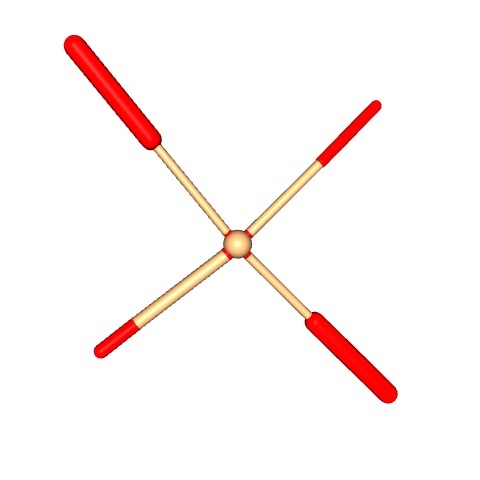
\includegraphics[width=0.9\linewidth]{./resources/ant_307.png}
            \caption{Example of an ant in the environment. The red legs depict the lower leg part, and the light beige represents the upper leg part.}
            \label{fig:ant_env}
        \end{figure}
        To evolve a generalist MC-pair, we have to enable the ant to modify its morphology. Each leg part is parameterized by two attributes: length and width, resulting in a total of 16 distinct morphological parameters. The leg lengths are constrained between 0.1 and 1.5, while the widths are limited from 0.08 to 0.2. 
        
        To ensure a fast and successfull experiment, additional modifications to the ant's environment were necessary. Normally, the simulation would terminate the when the ant's torso ascends or descends to a specific height. This range has been increased to allow the ant to grow longer legs. Furthermore, additional settings were introduced to terminate the run whenever no significant forward movement was detected, suggesting that the ant had frozen in place. Another custom rule was implemented to detect if the ant flipped upside down by monitoring the z-vector of the torso. These additions significantly reduced evaluation times, especially at the start of the evolutionary process.

    \subsection{Experimental parameters}
        For the controller, a fully connected feedforward ANN is evolved, based on the topology used by Triebold et al. \cite{Corinna_Triebold}. This topology consists of a single hidden layer with 20 neurons. The input layer corresponds to the ant's continuous observation space, which includes 27 observations, such as the angles between the torso and leg connections or velocity values, resulting in 27 input nodes. The output layer corresponds to the ant's action space, where actions are values ranging from [-1, 1], representing the torque applied to the rotors. This results in a total of 8 actions and thus 8 output nodes. Each layer also includes a bias node.
        
        For the parameters used in the XNES algorithm, we used the default settings provided by the algorithm. The initial standard deviation of the search was set to 0.01, and the initial parameter ranges for the controller and encoded morphology parameters were [-0.1, 0.1]. To decode the morphology parameters, a linear transformation is used where the lower bound morphology constraint maps to -0.1 and the upper bound morphology constraint maps to 0.1. The lower and upper bound constraints used for the length and width of the legs are [0.1, 1.5] [0.05, 0.2] respectively. \textbf{Should I also insert these linear transformation formula's that I used specifically?}
        
        The parameters used for the penalty function were decided based on initial experimental analysis. For the growth rate $r^i$, we settled on 1.03 in conjunction with two scale factors for $\alpha$. This means we are using two different penalty functions. The reason for this is that when the morphological parameters are decoded into negative values, the environment will crash because it cannot accommodate negative values for morphology. In these cases, $\alpha$ is set to 1000; otherwise, it is set to 100.
        
        For the evolutionary process, we decided to evaluate the generalist scores after 2500 generations, instead of at every generation from the start. The reason for this is to decrease computational cost, but primarly because at the start of the evolutionary process, it is difficult to achieve high fitness scores due to the search for an effective morphology to exploit. After 2500 generations, a generalist score will be computed from the fittest individual in each generation. If there is no improvement found after 500 generations, the process is either terminated or a partition will occur.

        Additionaly, we conducted an alternative evolutionary run in which partitioning was disabled, allowing the run to extend to 5000 generations. The reason for this is because the of the unpredictability of discovering a generalist MC-pair, due to it not being the objective function, but a secondary outcome of the method used. The exclusion of paritioning in this scenario will provide a valuable basis for comparison with the partitioned approach.
    \subsection{Training, evaluation and testing}
        The MC-pair's training consists of different simulated environments, where the terrain is algorithmically generated based on the inputs. In this experiment, we consider three different environments. The first environment, referred to as the default environment, is a single static environment with a flat surface. The two remaining environments are dynamically generated, named the rough terrain environment and the hill terrain environment (see Figure~\ref{fig:rough_terrain} and Figure~\ref{fig:hills_terrain}, respectively). The rough terrain environment is generated based on the block size and floor height. The block size determines the size of a block that can be elevated, and the floor height determines the range at which this block can be elevated. For the hill terrain environment, we utilize a Perlin noise map to determine the elevations of the terrain. The scale parameter determines the smoothness of the terrain, meaning that the terrain heights have smaller and subtler changes in height, leading to a more hilly terrain, with the floor height serving as the range at which these heights can be set. 
        \begin{figure}[ht]
            \centering
            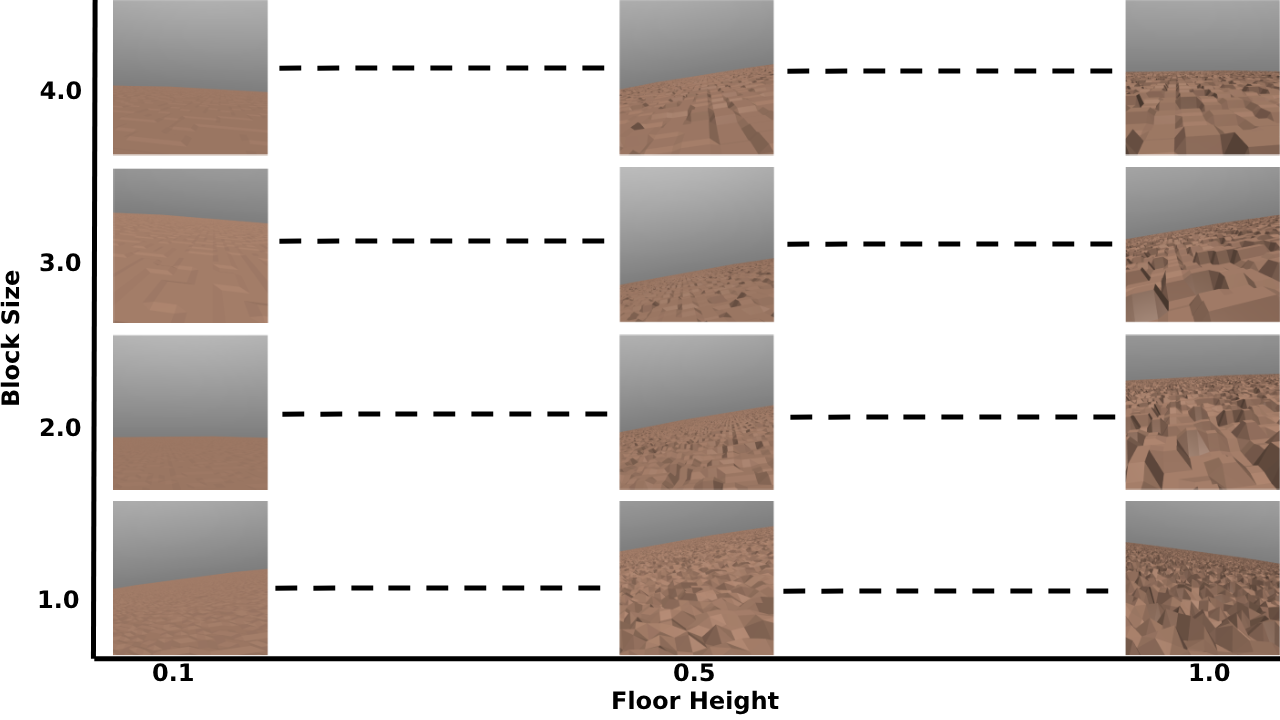
\includegraphics[width=\linewidth]{./resources/rough_terrain.png}
            \caption{Rough terrain environment generation, based on the block size and floor height.}
            \label{fig:rough_terrain}
        \end{figure}
        \begin{figure}[ht]
            \centering
            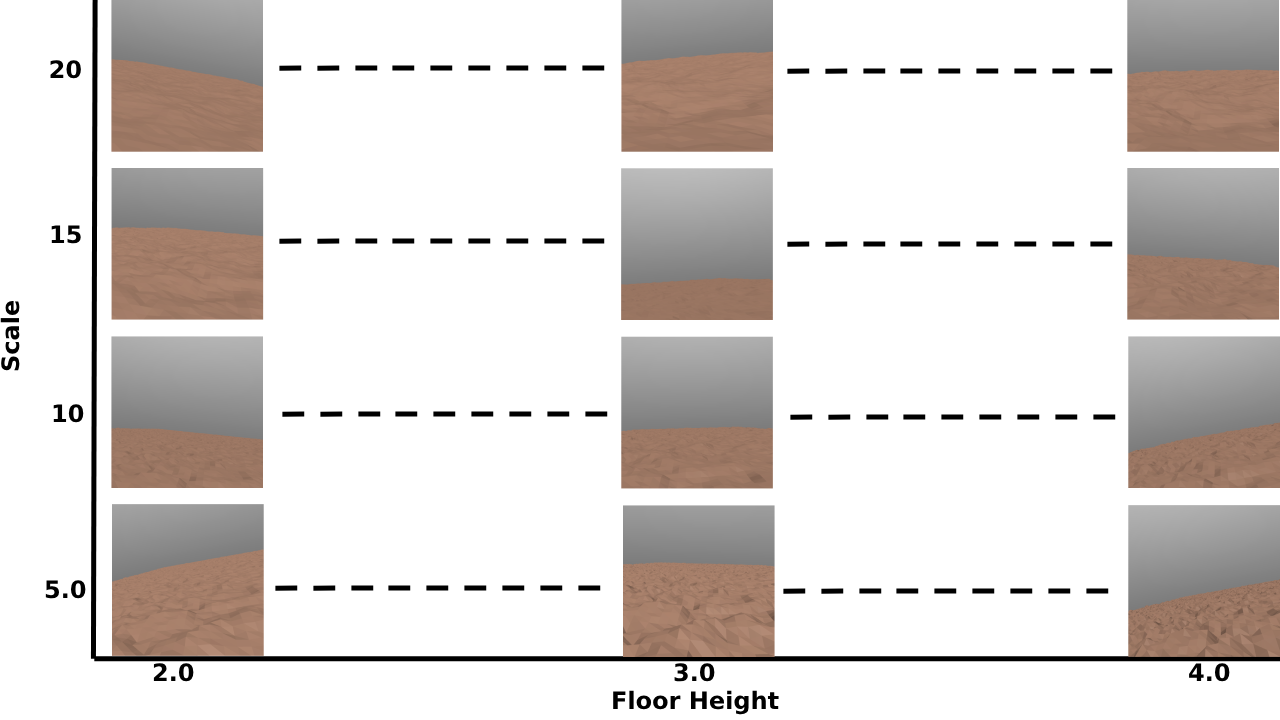
\includegraphics[width=\linewidth]{./resources/hills_terrain.png}
            \caption{Hills terrain environment generation, based on the scale of the Perlin noise and floor height.}
            \label{fig:hills_terrain}
        \end{figure}

        In total, we have 40 variations of the rough terrain environment, 44 variations of the hill terrain environment, and the default environment, totaling up to a set of 85 different environments. We will split this set into training, validation, and testing sets. In our case, for the validation set, we will use the same set as for the training set. The training set contains the default environment, 24 hill environments, and 24 rough terrain environments, totaling to 49 environments. The testing set contains 20 hill environments and 16 rough terrain environments, totaling to 36 environments. The exact splits are shown in Table~\ref{tab:split_table}.

        To test the generalizability of the MC-pair, we run two separate tests. The first test is to evaluate the performance on environments similar to those of training, with both the testing and training environment parameters drawn from the same distribution, which we call interpolation. The second test is to evaluate the performance on environments different from those of training, with the testing and training environment parameters drawn from separate distributions, which we call extrapolation. In summary, to test interpolation, we will utilize the training set, and to test extrapolation, we will use the testing set described in Table~\ref{tab:split_table}.

        \begin{table*}[ht]
            \centering
            \caption{This table shows the environment set splits and used ranges for the hill and rough environments.}
            \begin{tabular}{|c|c|c|c|c|}
            \hline
            \textbf{Environment} & \textbf{Parameters} & \textbf{Training Set} & \textbf{Testing Set} & \textbf{Step} \\ \hline
                Rough terrain & 
                \makecell{Block size \\ Floor height} & 
                \makecell{$[1, 4]$ \\ $[0.2, 0.4] \cup [0.7, 0.9]$} & 
                \makecell{$[1, 4]$ \\ $[0.1] \cup [0.5, 0.6] \cup [1.0]$} & 
                \makecell{1 \\ 0.1}
            \\ \hline
                Hills terrain &
                \makecell{Scale \\ Floor height} & 
                \makecell{$[5, 20]$ \\ $[2.2, 2.6] \cup [3.4, 3.8]$} & 
                \makecell{$[5, 20]$ \\ $[2.0] \cup [2.8, 3.2] \cup [4.0]$} & 
                \makecell{5 \\ 0.2}
            \\ \hline
        \end{tabular}
        \label{tab:split_table}
        \end{table*}
\section{Results}
    In this section, we will present the results of all three experiments. In the heatmaps, the by red enclosed cells indicates the environments from the testing set used for extrapolation testing, while the non-red-enclosed cells represent the environments from the training set used for interpolation testing. Lastly, we will present the results on the different types of morphologies evolved in our experiments. Visualizations of these evolved MC-pairs from our different experiments can be viewed online\footnote{See the visual demonstration of the behaviors of the MC-pairs at: \url{https://www.youtube.com/watch?v=CWxKFhSb94I}}.
    \subsection{Experiment 1: One generalist}
        \begin{figure*}[!ht]
            \centering
            \begin{subfigure}{\textwidth}
                \centering
                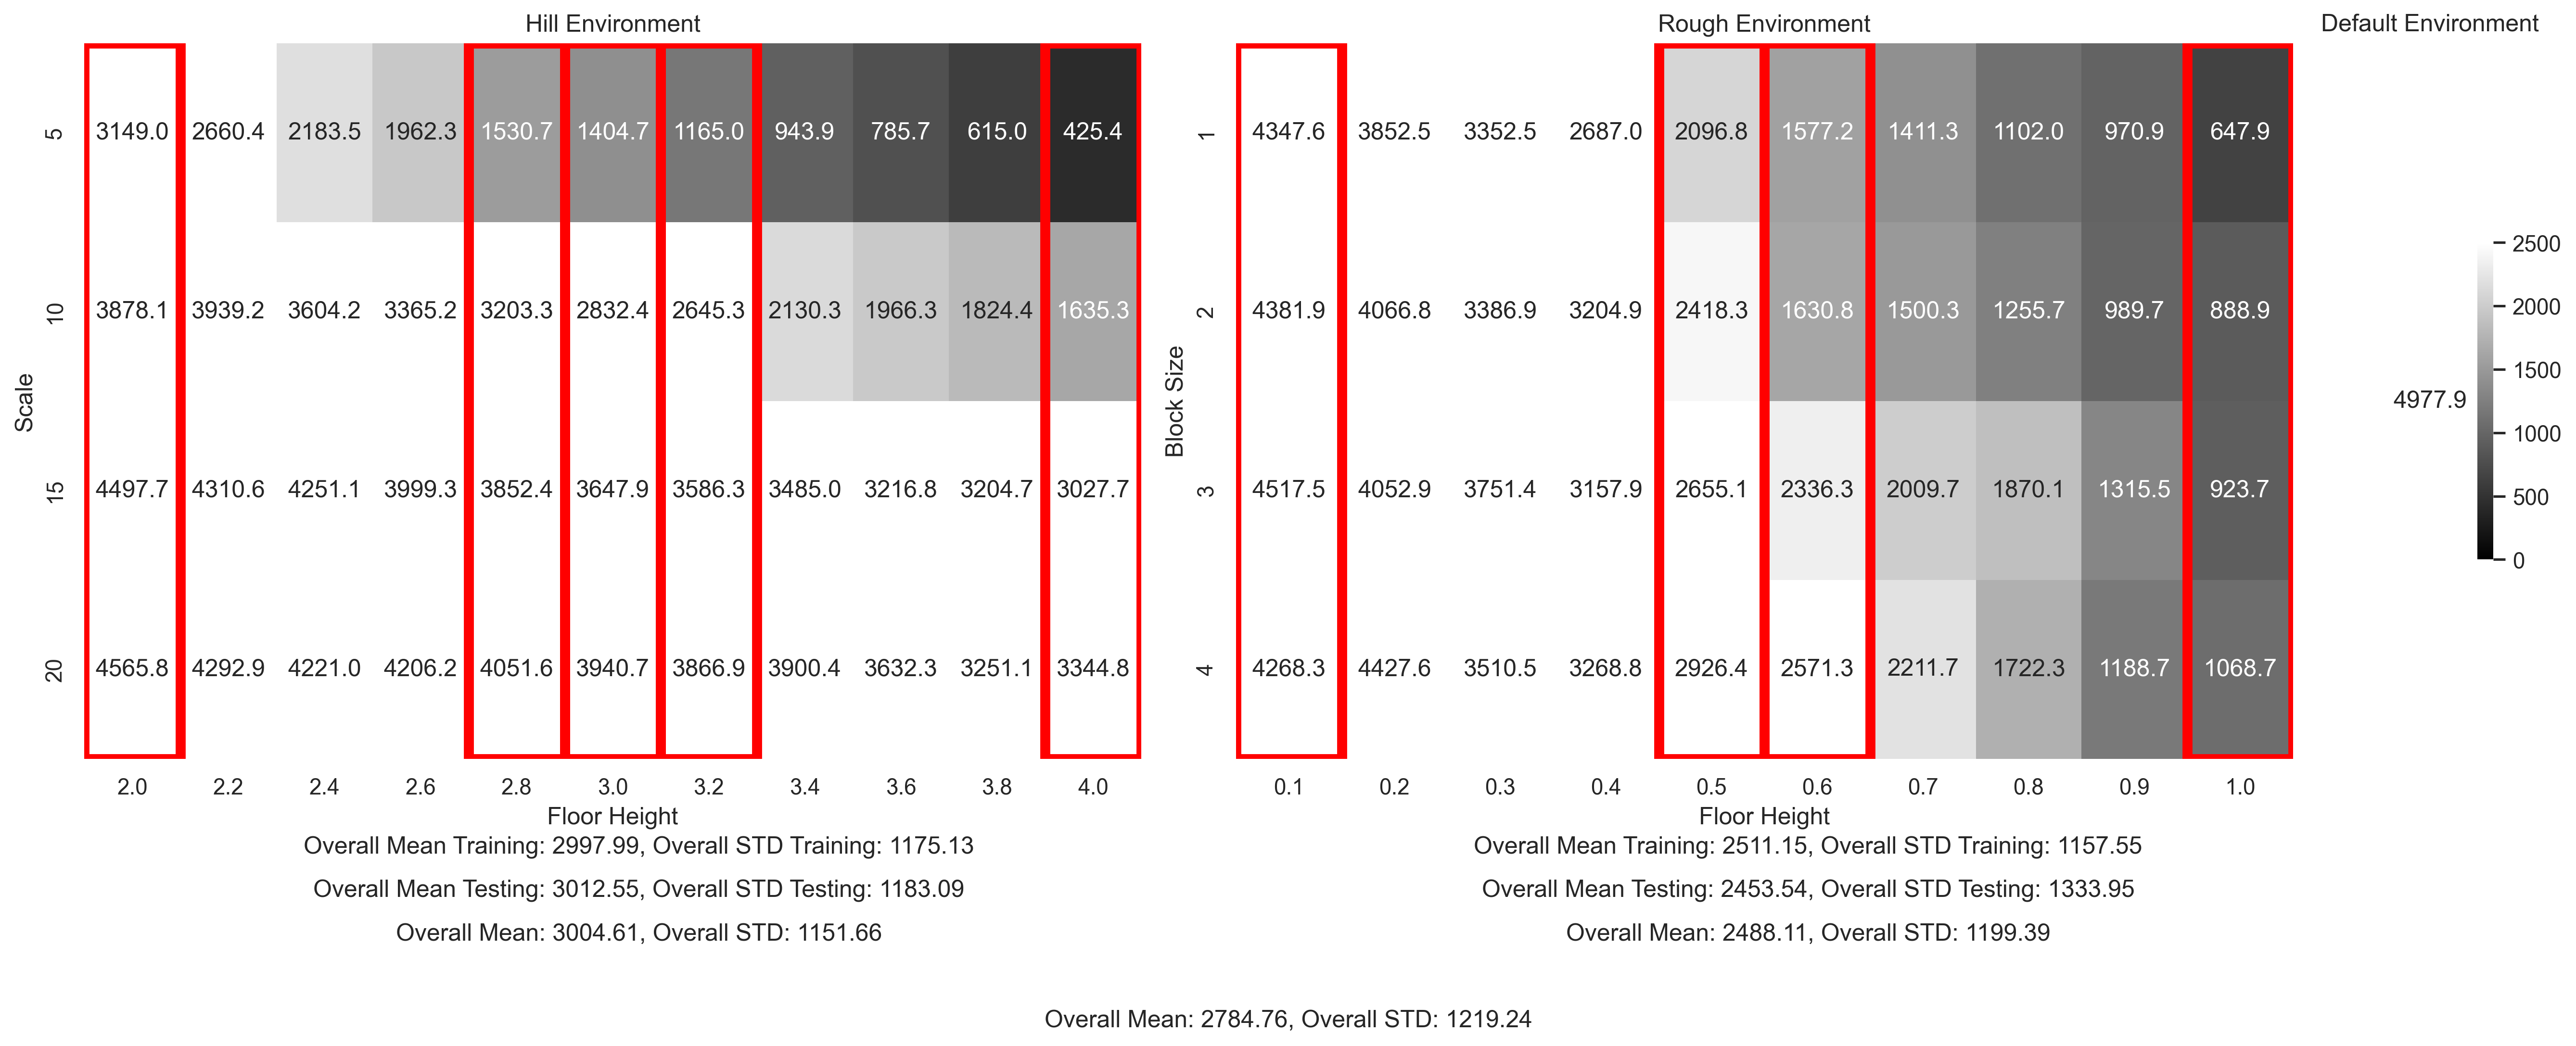
\includegraphics[width=\linewidth]{./resources/generalist_4_2784/fitness_heatmap.png}
                \caption{Fitness heatmap from one generalist MC-pair evolved over 5000 generations with partitions disabled}
                \label{fig:fit_heat_generalist}
            \end{subfigure}

            \begin{subfigure}{\textwidth}
                \centering
                \begin{minipage}{0.19\textwidth}
                    \centering
                    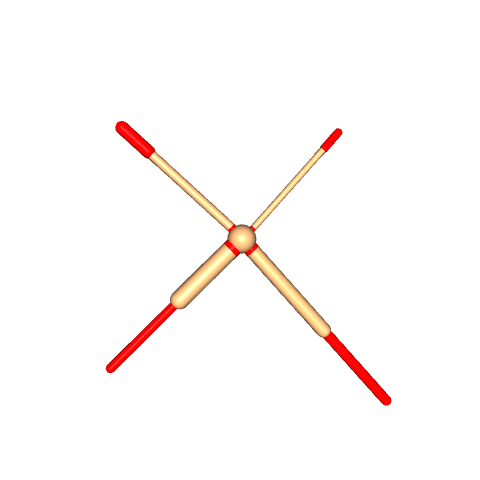
\includegraphics[width=\linewidth]{resources/generalist_2_2350/ant.png}
                    \textbf{2350}
                \end{minipage}
                \hfill
                \begin{minipage}{0.19\textwidth}
                    \centering
                    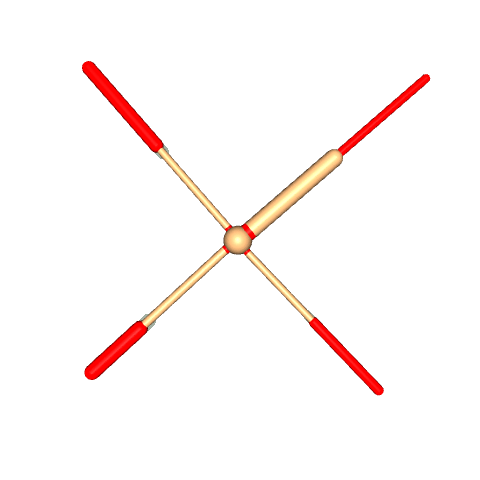
\includegraphics[width=\linewidth]{resources/generalist_3_2412/ant.png}
                    \textbf{2412}
                \end{minipage}
                \hfill
                \begin{minipage}{0.19\textwidth}
                    \centering
                    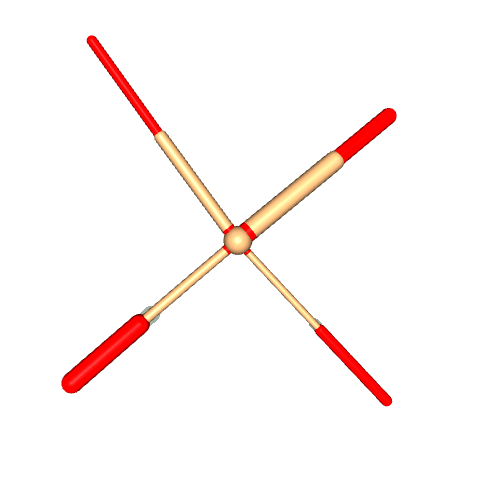
\includegraphics[width=\linewidth]{resources/generalist_4_2784/ant.png}
                    \textbf{2784}
                \end{minipage}
                \hfill
                \begin{minipage}{0.19\textwidth}
                    \centering
                    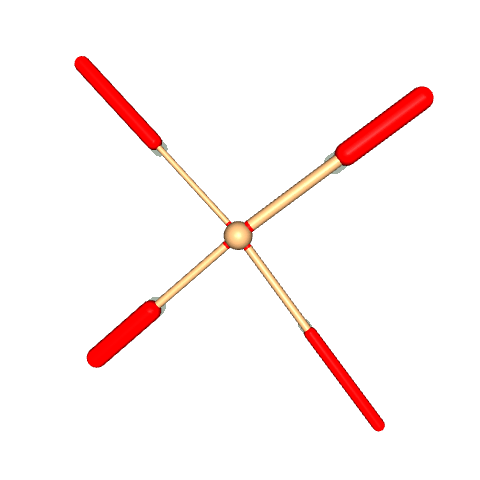
\includegraphics[width=\linewidth]{resources/generalist_1_2966/ant.png}
                    \textbf{2966}
                \end{minipage}
                \hfill
                \begin{minipage}{0.19\textwidth}
                    \centering
                    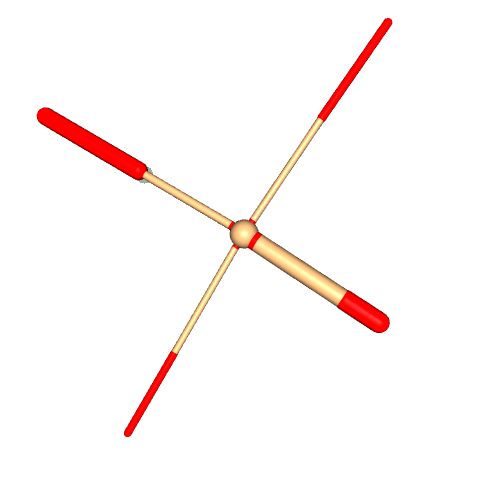
\includegraphics[width=\linewidth]{resources/generalist_5_3126/ant.png}
                    \textbf{3126}
                \end{minipage}

                \caption{Morphology evolved for one generalist MC-pair from different evolutionary runs ordered by generalist score, which is shown below the image.}
                \label{fig:gen_ant_images}
            \end{subfigure}
            
            \begin{subfigure}{\textwidth}
                \centering
                \begin{minipage}{0.32\textwidth}
                    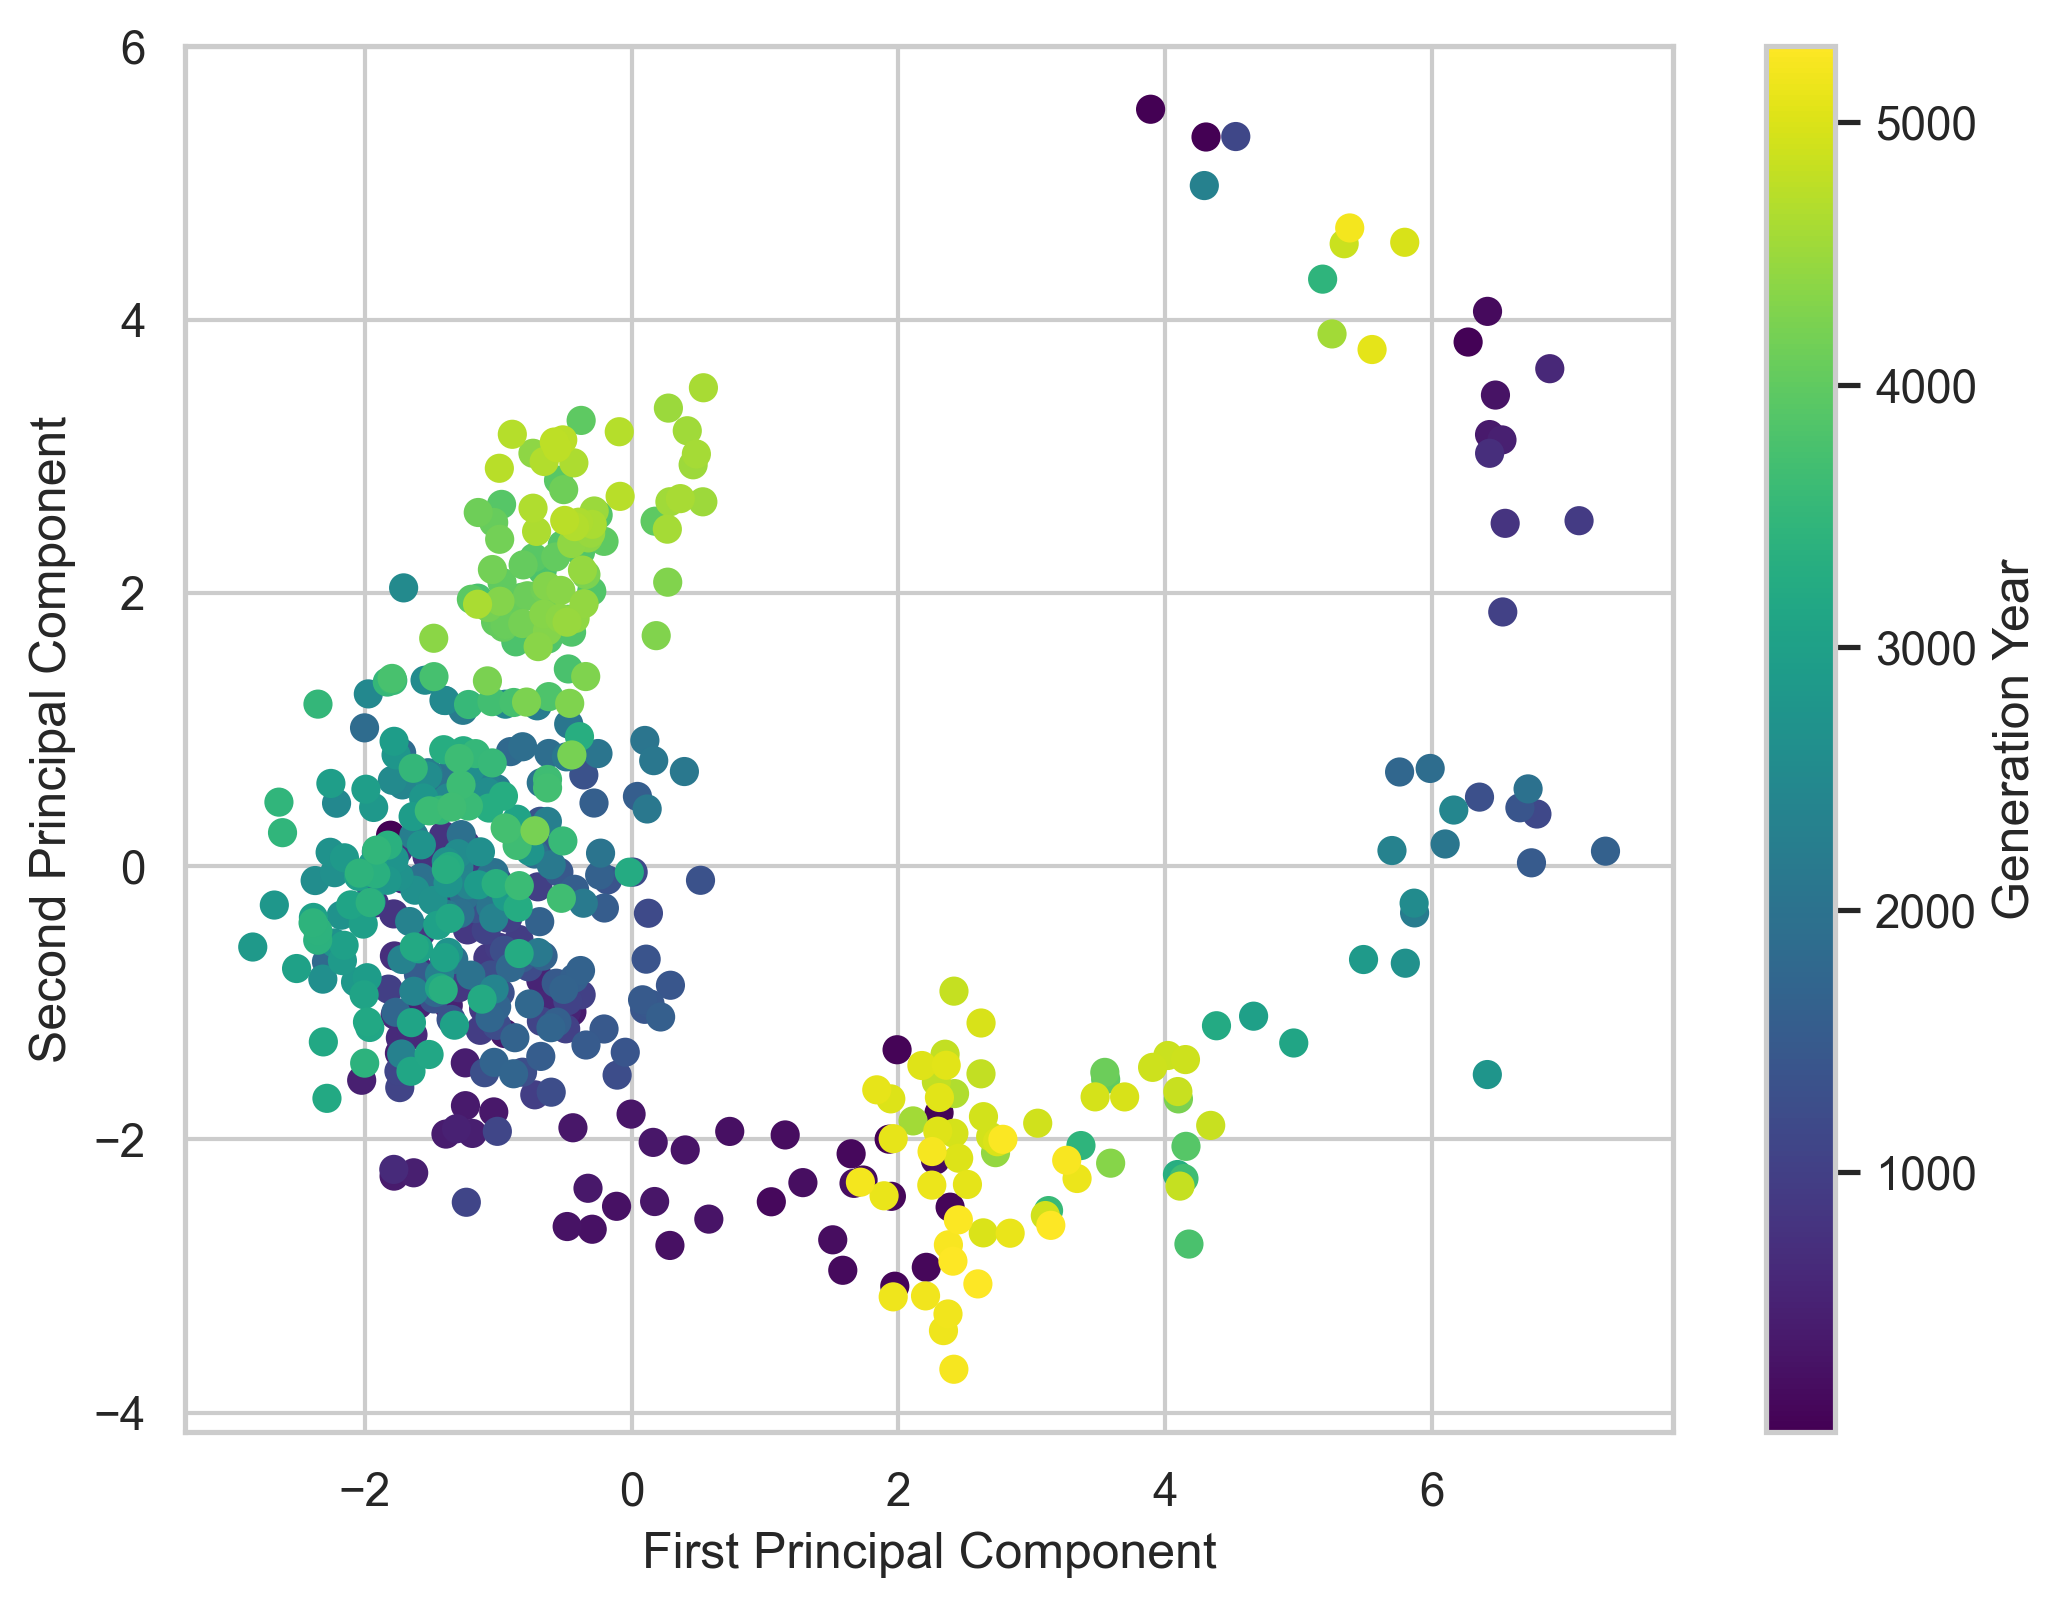
\includegraphics[width=\textwidth]{./resources/generalist_3_2412/pca_scatterplot.png}
                    \centering
                    \textbf{2412}
                \end{minipage}
                \hfill
                \begin{minipage}{0.32\textwidth}
                    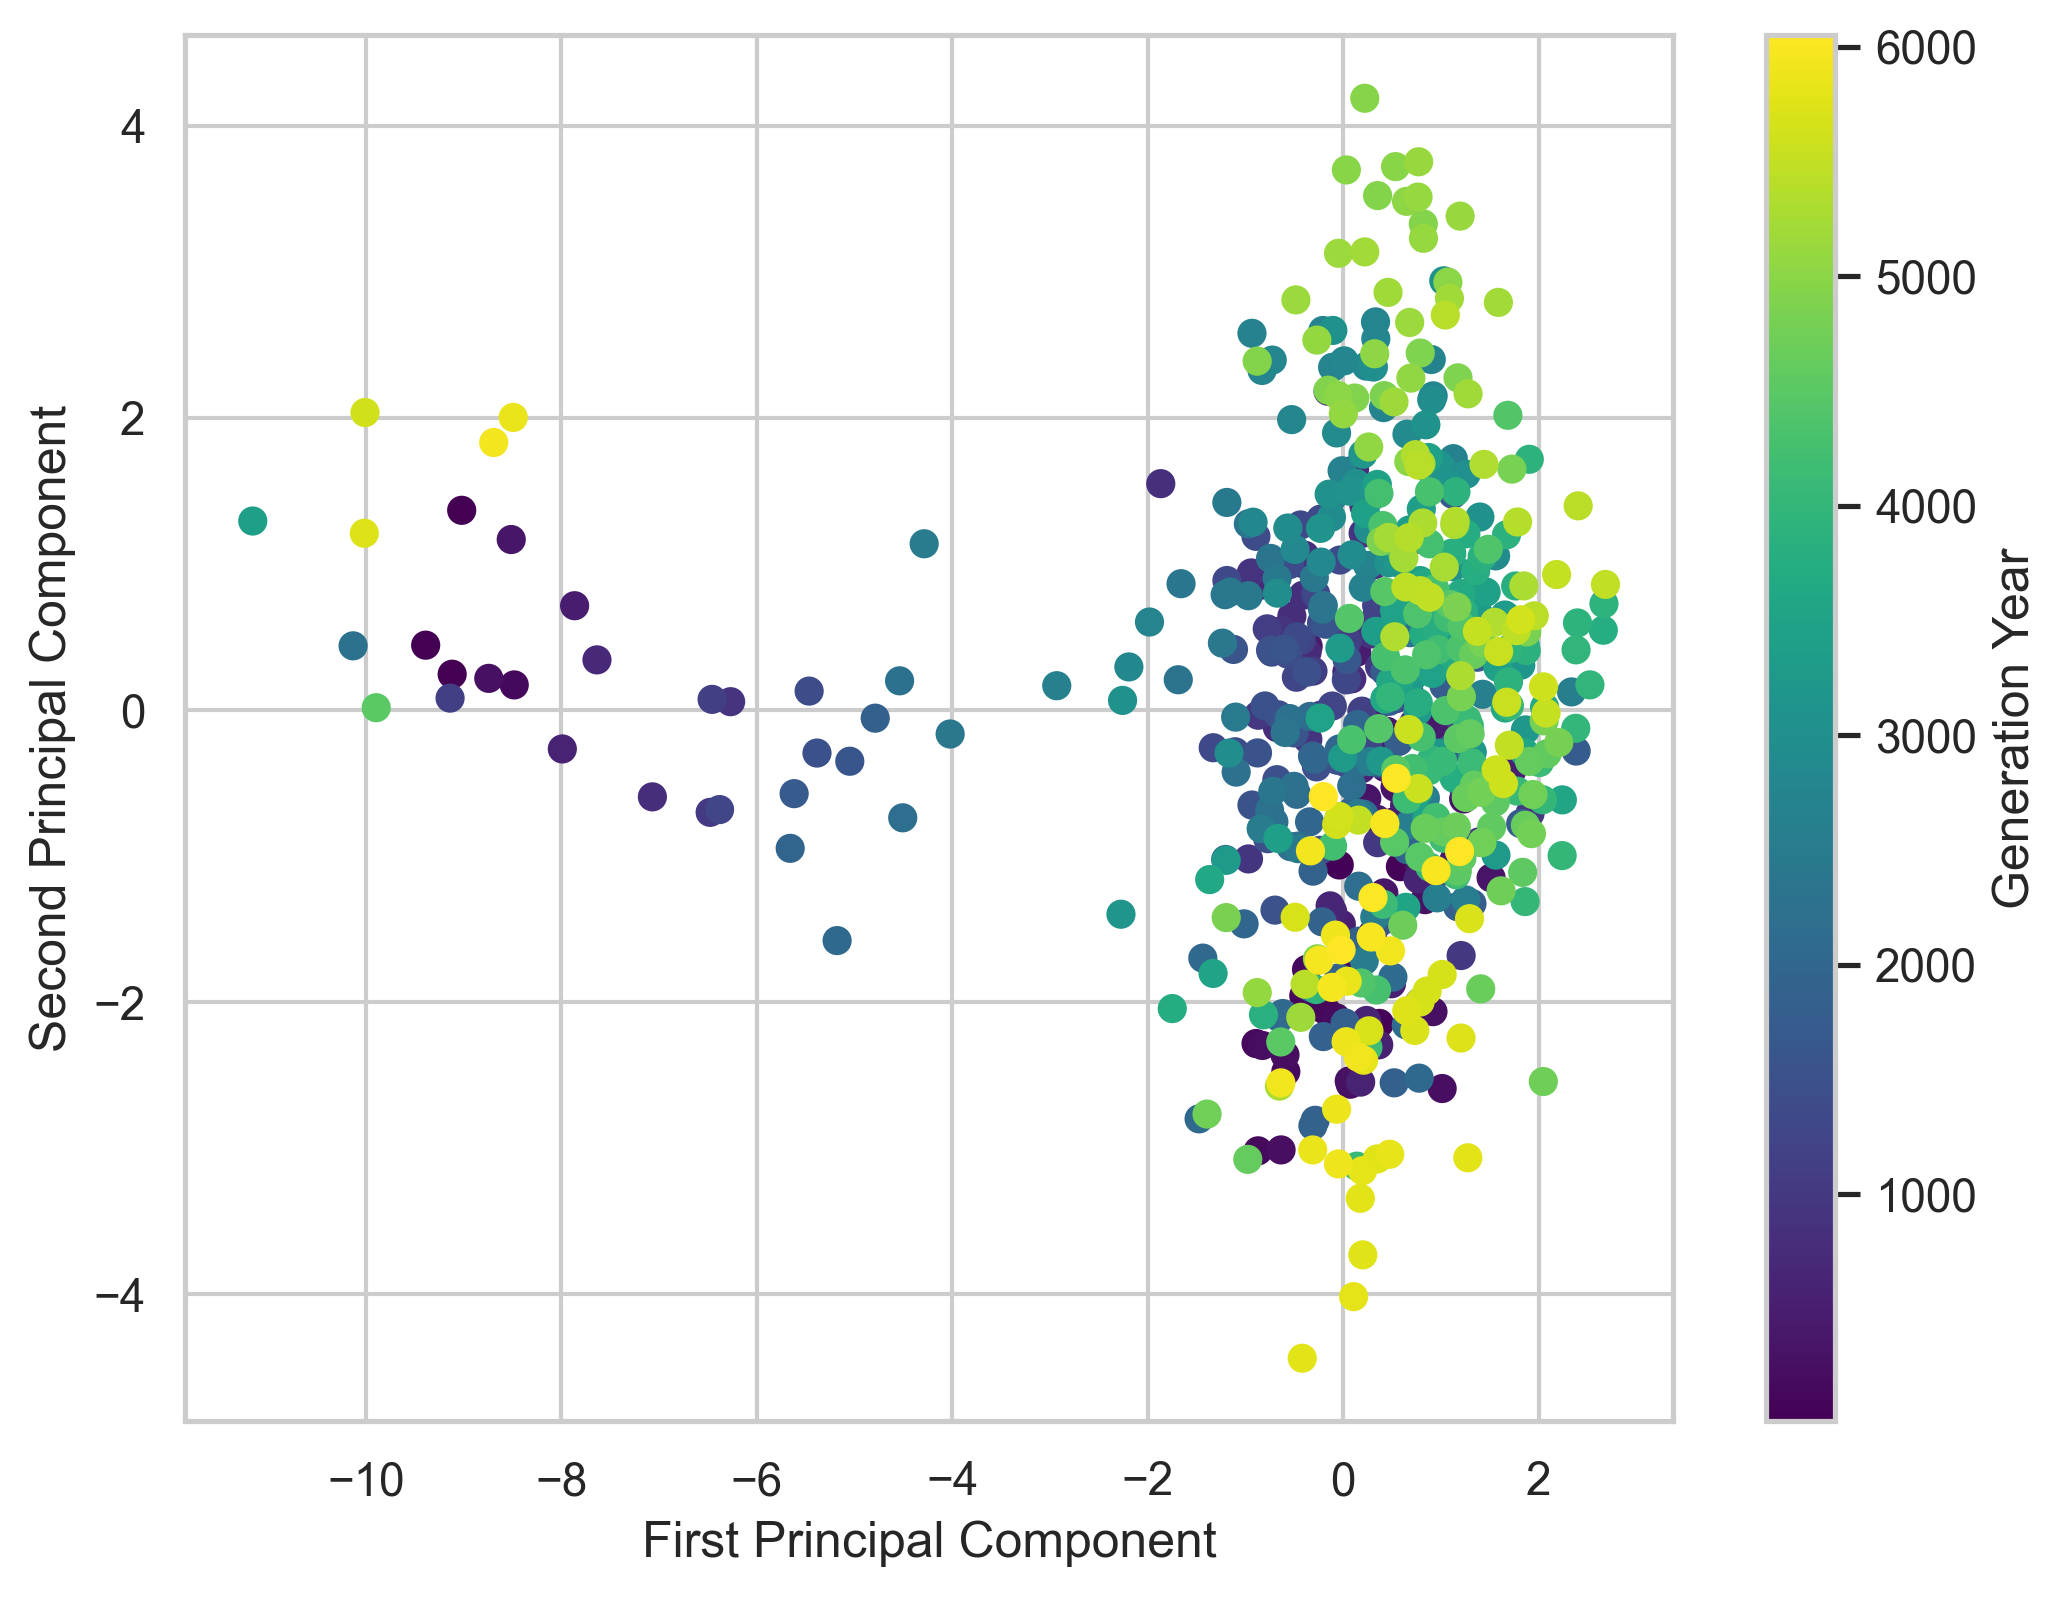
\includegraphics[width=\textwidth]{./resources/generalist_4_2784/pca_scatterplot.png}
                    \centering
                    \textbf{2784}
                \end{minipage}
                \hfill
                \begin{minipage}{0.32\textwidth}
                    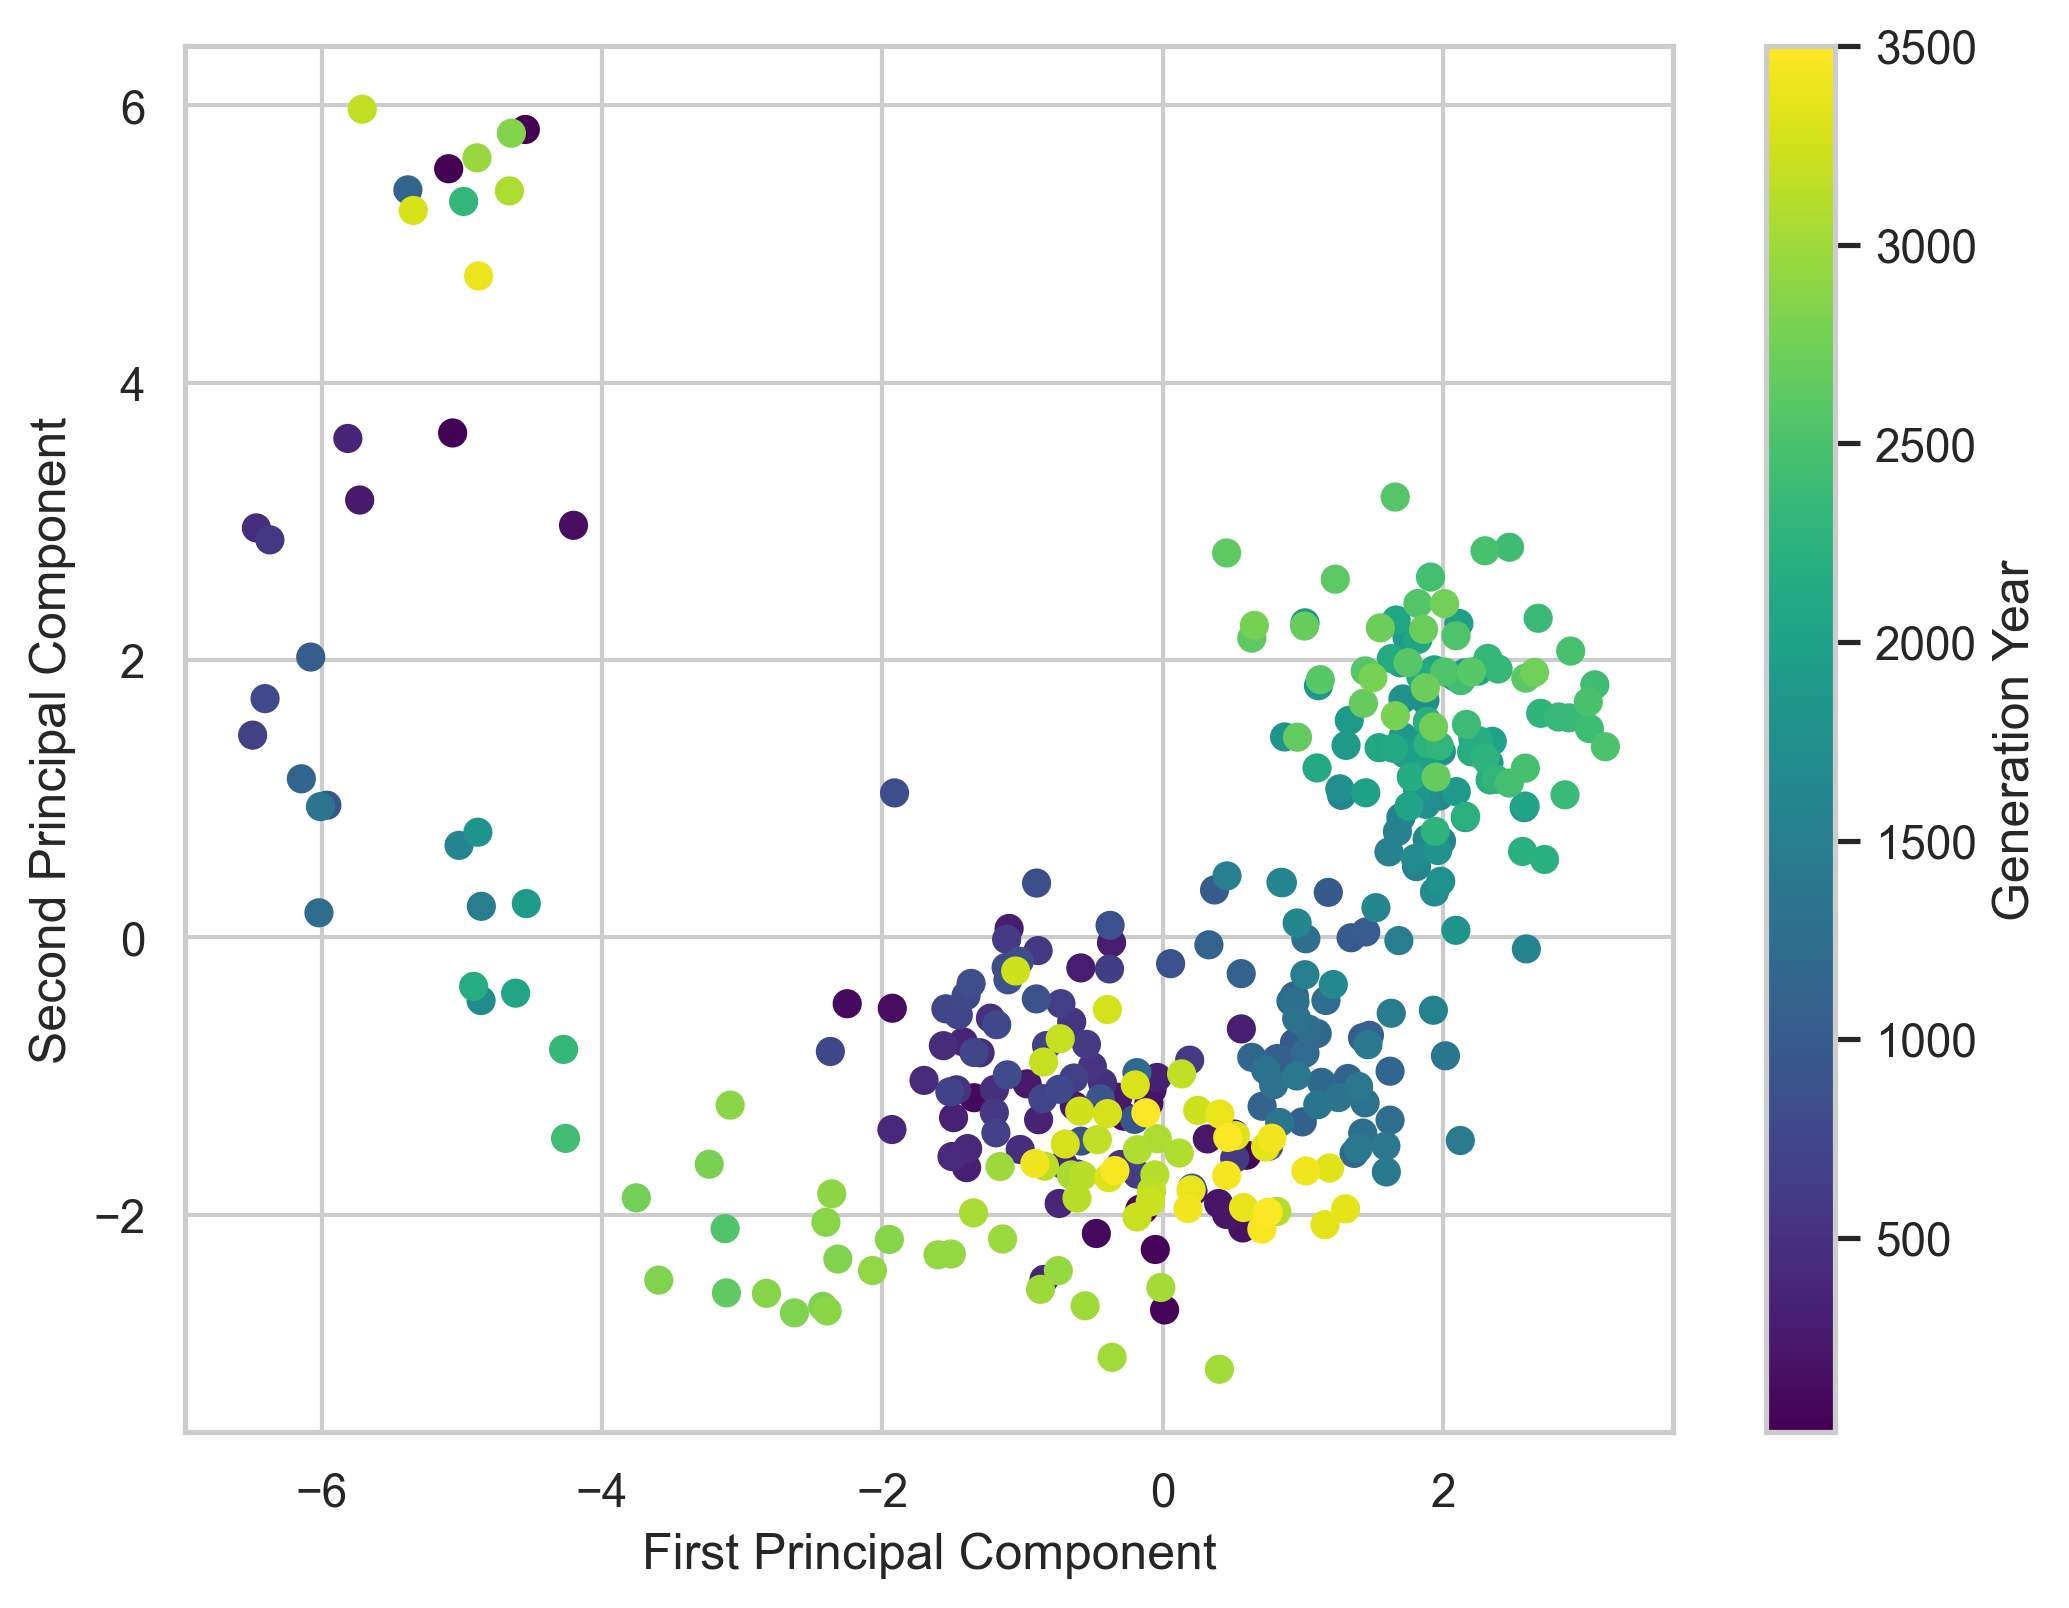
\includegraphics[width=\textwidth]{./resources/generalist_5_3126/pca_scatterplot.png}
                    \centering
                    \textbf{3126}
                \end{minipage}
                \hfill
                \caption{PCA scatterplots where the morphological parameters are reduced to 2 principal components with generalist scores shown below.}
                \label{fig:pca_generalist}
            \end{subfigure}

            \caption{Experiment 1 - Results of the first experiment where we evolve one generalist MC-pairs to handle a wide range of diverse environments.}
            \label{fig:experiment1}
        \end{figure*}

        Figure~\ref{fig:fit_heat_generalist} shows the obtained fitness scores for each environment, represented in a heatmap for experiment 1. For the hill environment, the heatmap shows high performance in the environments at the lower left and relatively lower performance when nearing the the upper right. This may indicate inherint complexity in certain environments compared to others. The fitness scores and their standard deviations on the training and testing sets are similar. The training set has a mean fitness score of 2997.99 with a standard deviation of 1175.13, and the testing set has a mean fitness score of 3012.55 with a standard deviation of 1183.09. 
        
        For rough terrain environment, the heatmap also shows high performance in the environments at the lower left and relatively lower performance when nearing the upper right, but also more at the lower right part. The fitness scores and their standard deviations on the training and testing sets are also similar. The training set has a mean fitness score of 2511.15 with a standard deviation of 1157.55, and the testing set has a mean fitness score of 2453.54 with a standard deviation of 1333.95.
        
        A significant factor that determined the fitness score and the strategy utilized to achieve this score was the evolved morphology. In experiment 1, we conducted a total of five evolutionary runs, and the resulting MC-pairs are visible in Figure~\ref{fig:gen_ant_images}. These images are ordered by the generalist score obtained, which is shown below each image. The ants with generalist scores 2412, 2784, and 3126 have similar morphological structures and employed very similar strategies to move forward, using its two side legs accellerate itself forward. In contrast, the ant with generalist score 2966 uses a more conventional strategy, resembling more of how an actual ant would move.

        In order to to visualize the search for morphology, we employed principal component analysis (PCA) to reduce the dimensionality of the morphological parameters from 16 to 2 principal components, enabling us to plot them on a 2D graph. Figure~\ref{fig:pca_generalist} shows a scatterplot where each point represents a different morphology, with the color indicating the generation where that morphology was encountered and validated as the generalist. Across all three plots, there is no clear gradient towards a specific morphological structure, and morphological changes can even still occur very late in the evolutionary run. The scatterplots for generalist scores 2412 and 3126 shows that the search is happening within a circular-like space in the morphology space, whereas for generalist score 2784, the search begins with a morphology and tended to stick with its initialy generated morphology. 

    \subsection{Experiment 2: Partitioned generalist}
        \begin{figure*}[!htp]
            \centering
            \begin{subfigure}{\textwidth}
                \centering
                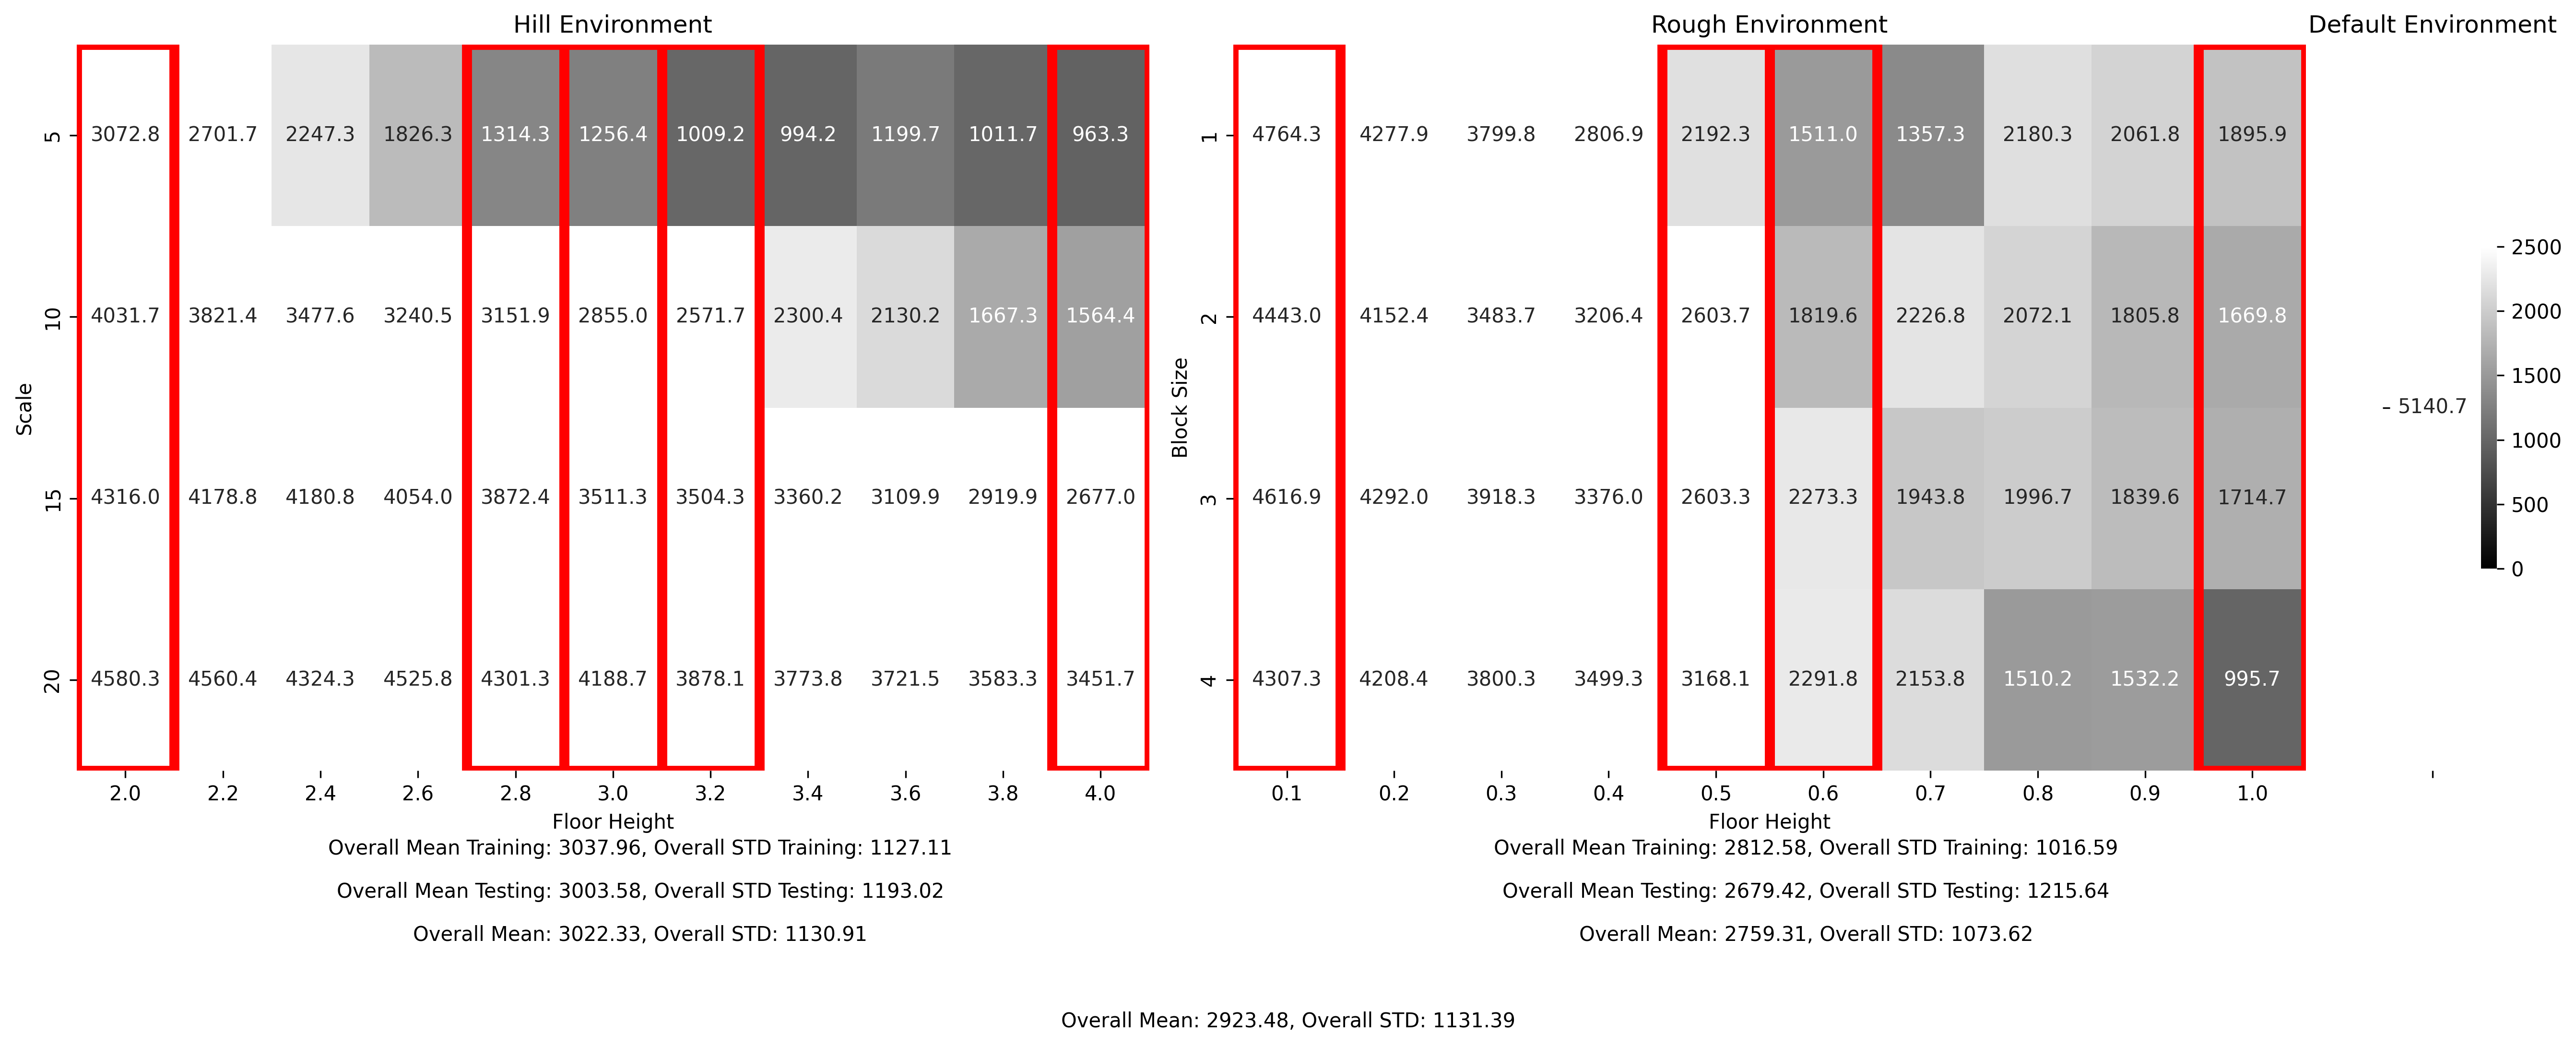
\includegraphics[width=\linewidth]{./resources/partition_5_2906_3/fitness_heatmap.png}
                \caption{Fitness heatmap of a set of generalist MC-pair}
                \label{fig:fit_heat_partitioned}
            \end{subfigure}

            \begin{subfigure}{\textwidth}
                \centering
                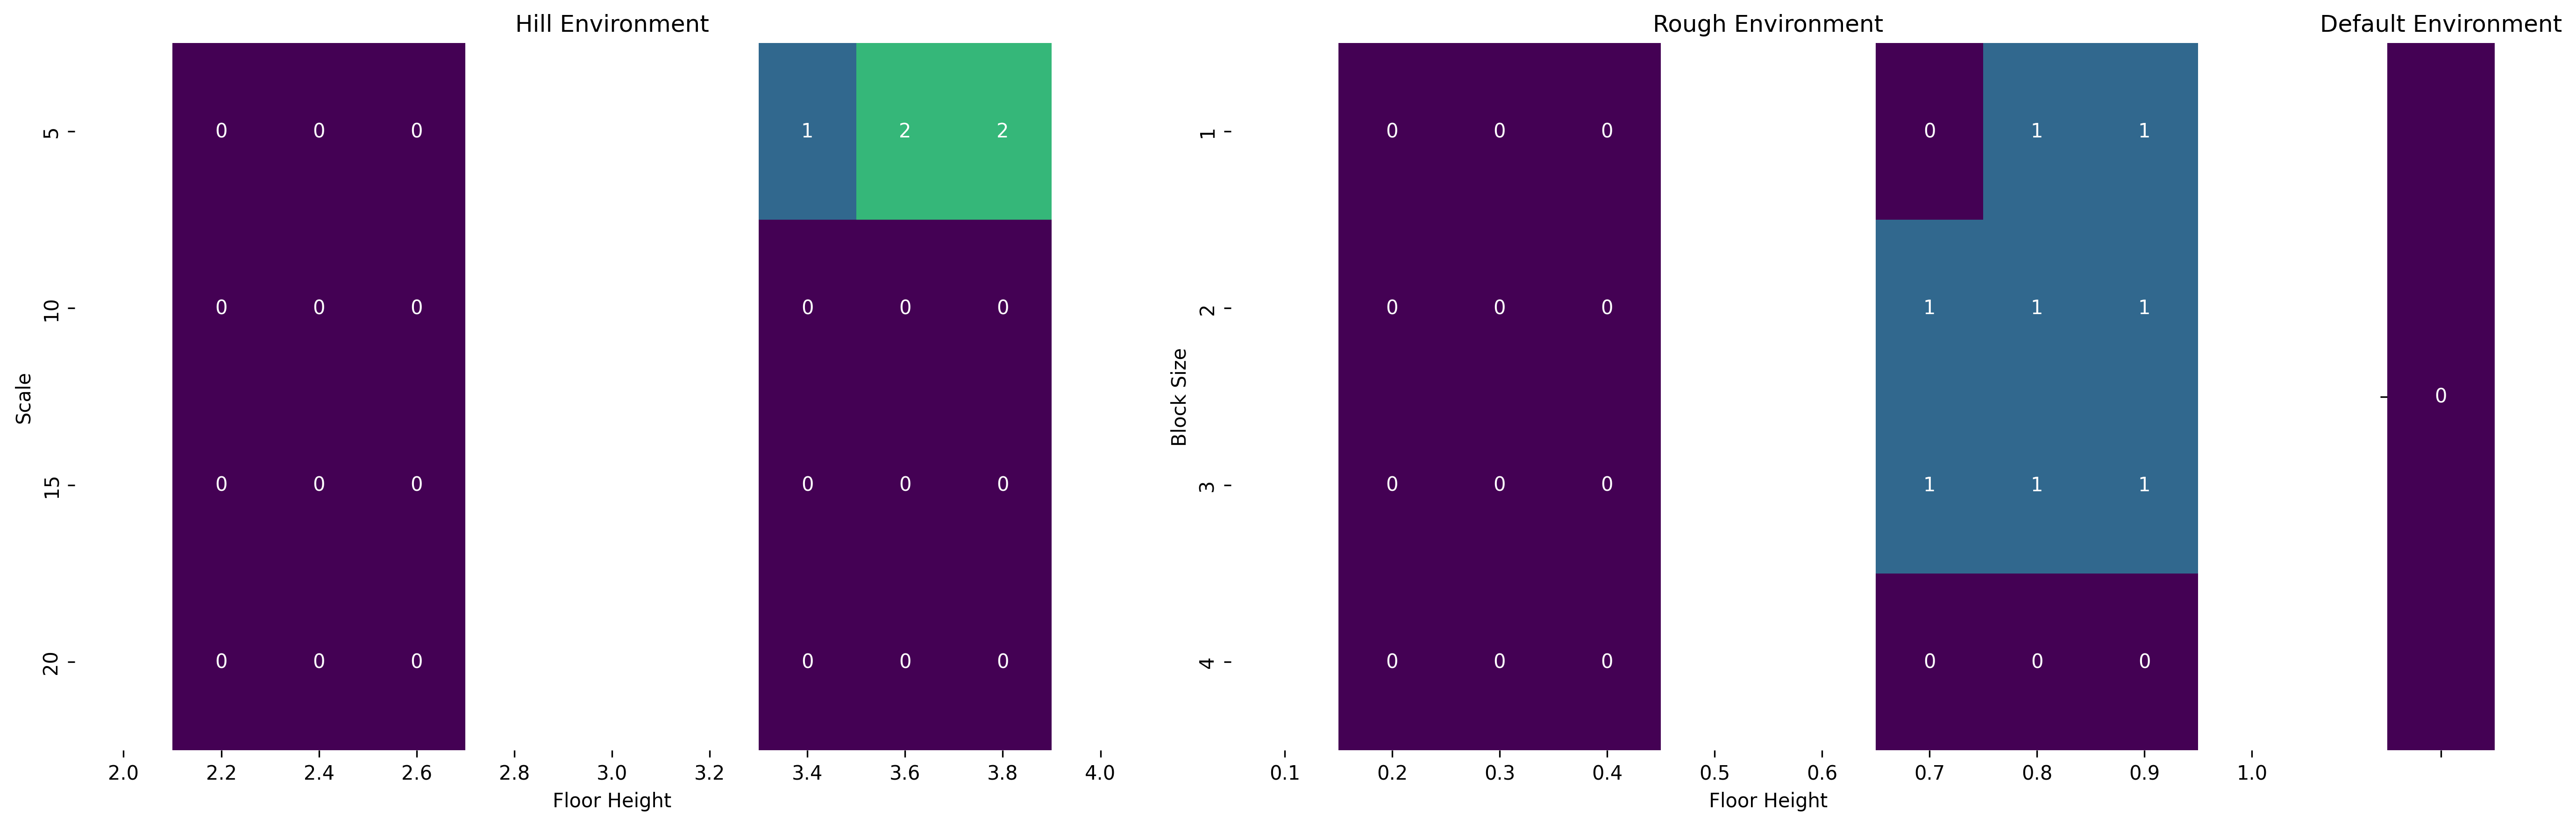
\includegraphics[width=\linewidth]{./resources/partition_5_2906_3/generalist_heatmap_partition.png}
                \caption{Figure showing to which partition the environment belongs to. In this experiment, three partitions where created.}
                \label{fig:heat_partition_number}
            \end{subfigure}

            \begin{subfigure}{\textwidth}
                \centering
                \begin{minipage}{0.19\textwidth}
                    \centering
                    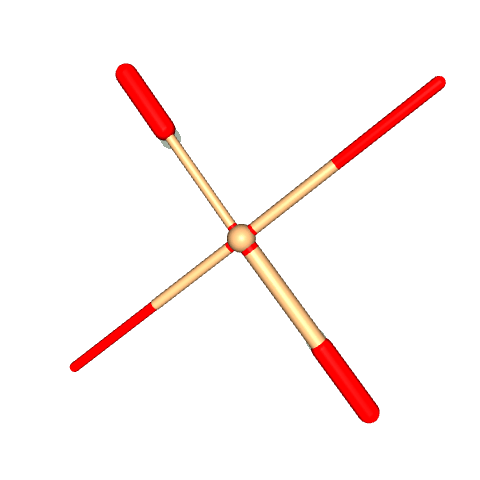
\includegraphics[width=\linewidth]{resources/partition_5_2906_3/ant_0.png}
                    \textbf{Partition 0}
                \end{minipage}
                \hfill
                \begin{minipage}{0.19\textwidth}
                    \centering
                    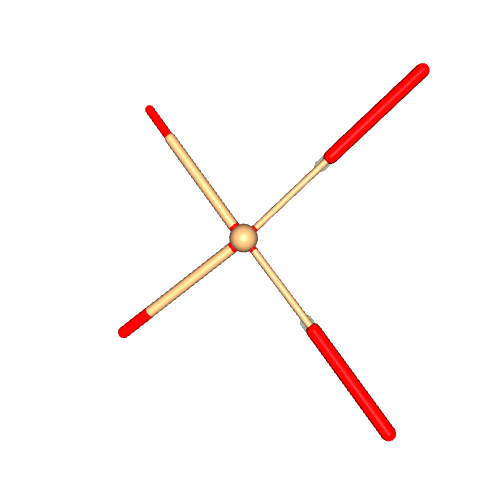
\includegraphics[width=\linewidth]{resources/partition_5_2906_3/ant_1.png}
                    \textbf{Partition 1}
                \end{minipage}
                \hfill
                \begin{minipage}{0.19\textwidth}
                    \centering
                    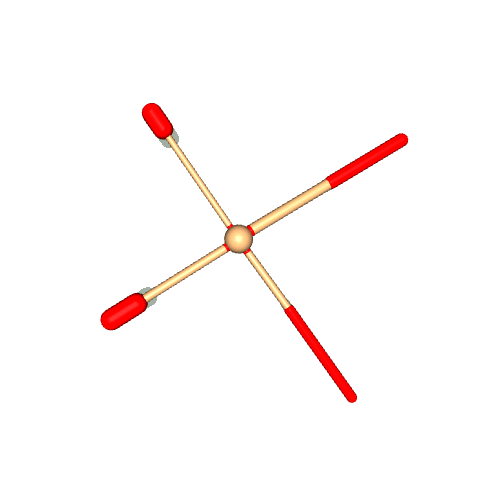
\includegraphics[width=\linewidth]{resources/partition_5_2906_3/ant_2.png}
                    \textbf{Partition 2}
                \end{minipage}
                \caption{Morphologies evolved for partitions of the environments}
                \label{fig:part_ant_images}
            \end{subfigure}

            \begin{subfigure}{\textwidth}
                \centering
                \begin{minipage}{0.32\textwidth}
                    \centering
                    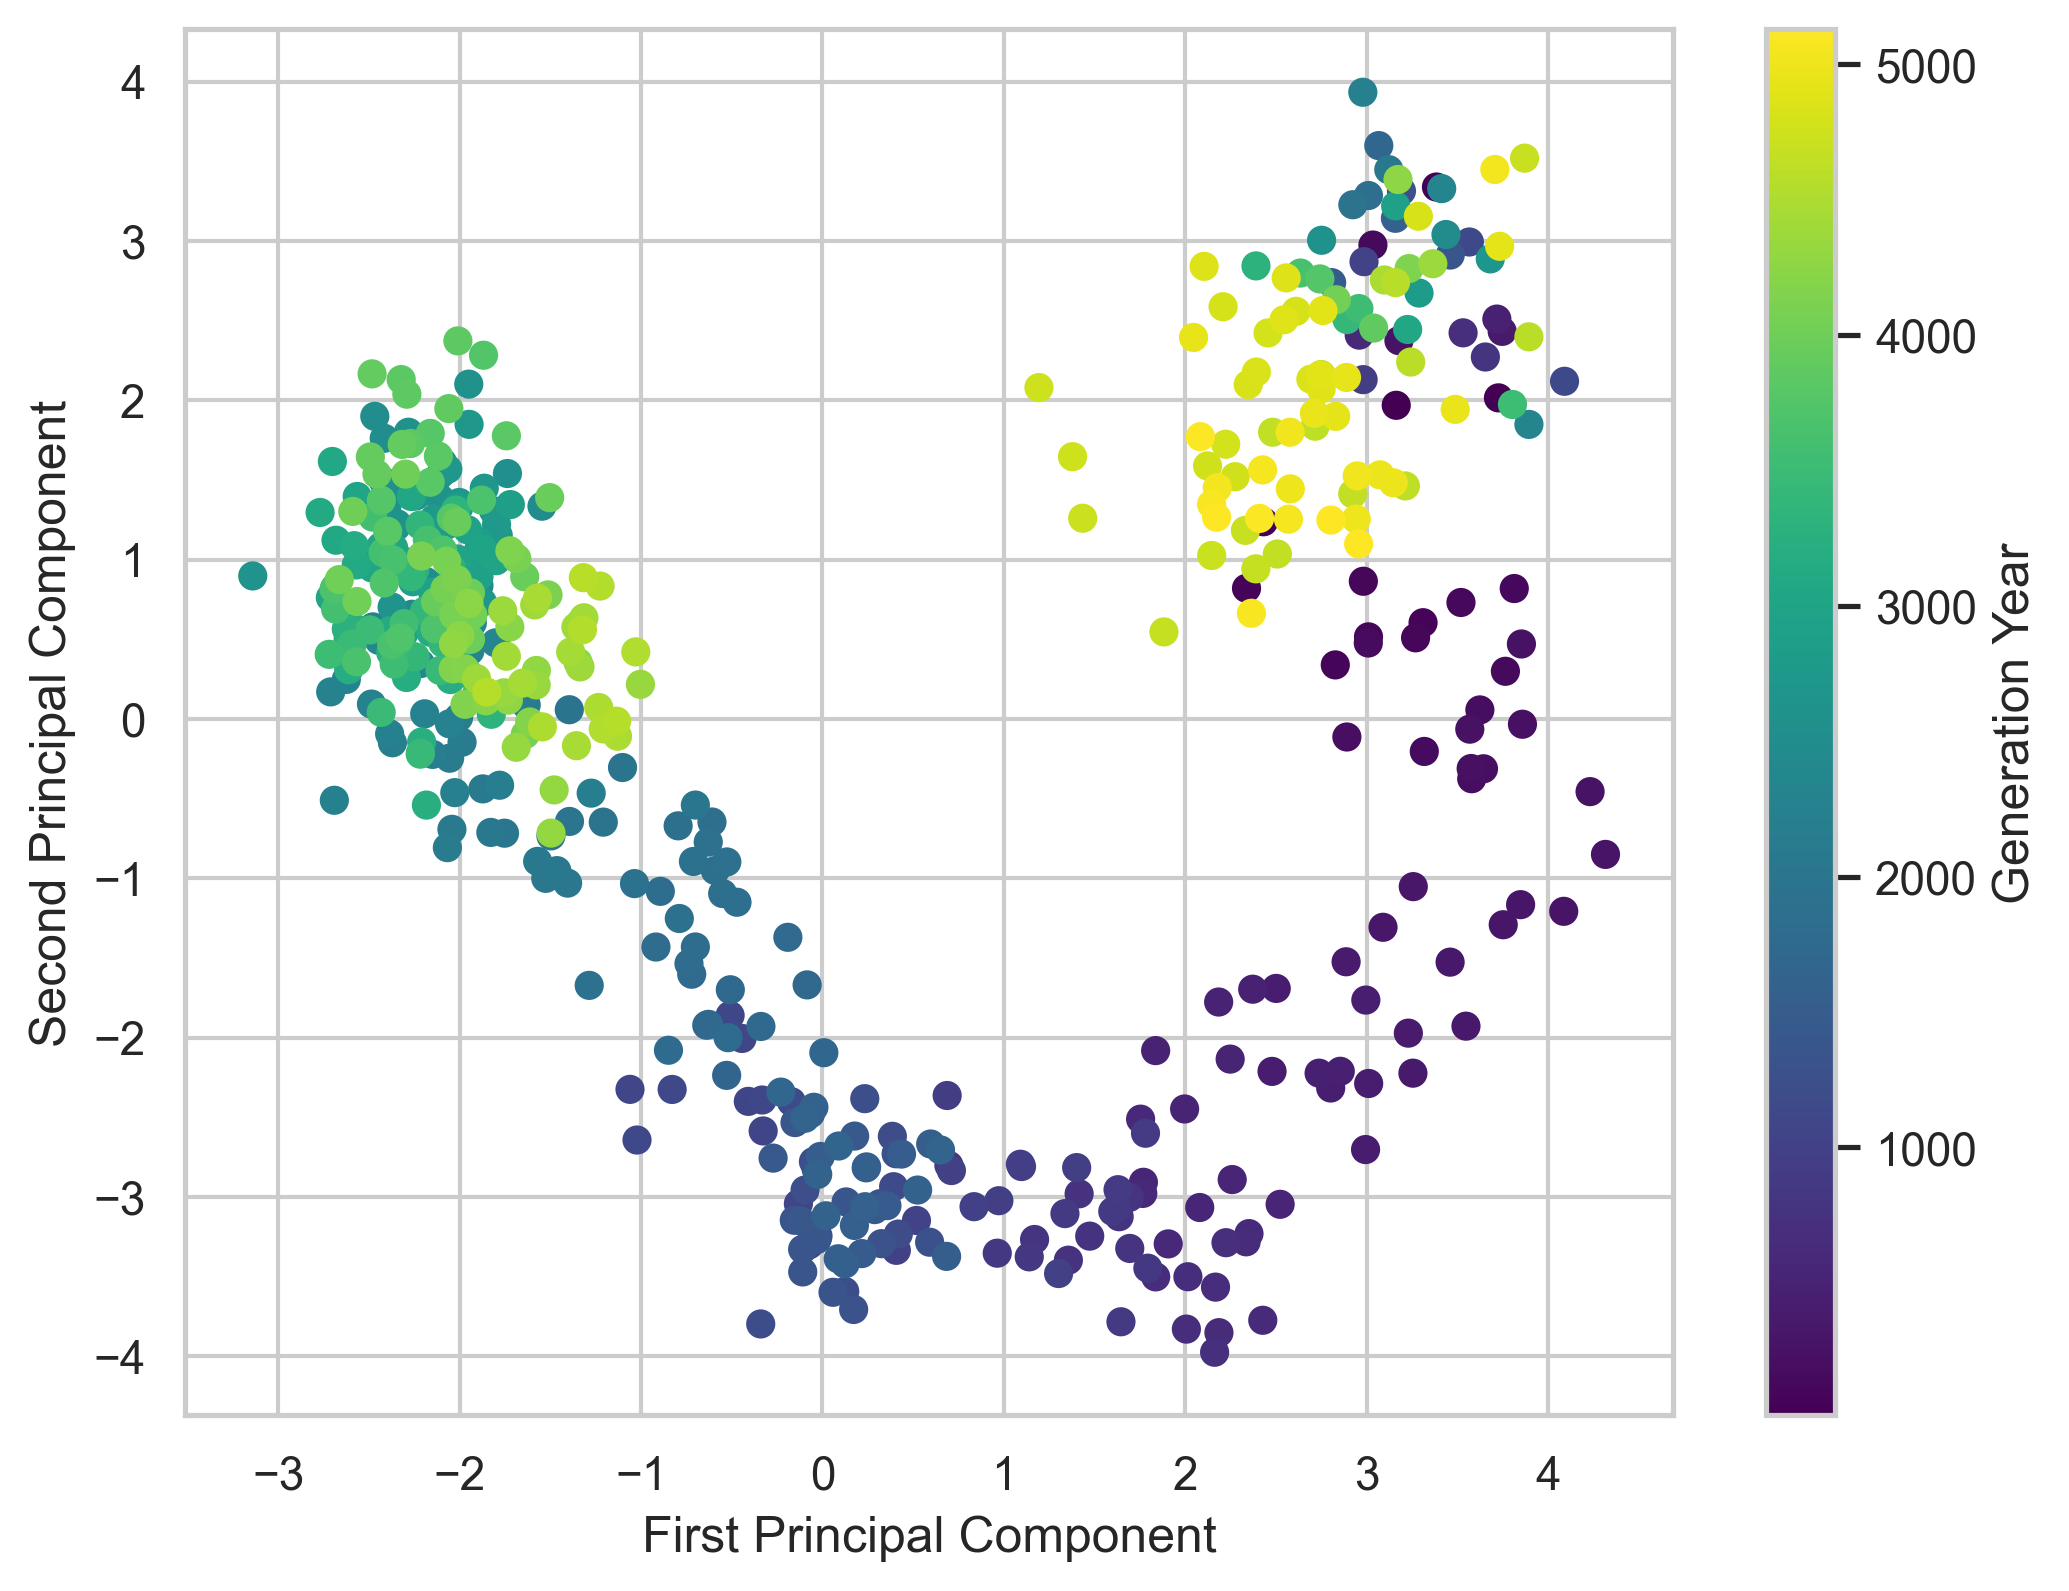
\includegraphics[width=\linewidth]{resources/partition_5_2906_3/partition_0/pca_scatterplot.png}
                    \textbf{Partition 0}
                \end{minipage}
                \hfill
                \begin{minipage}{0.32\textwidth}
                    \centering
                    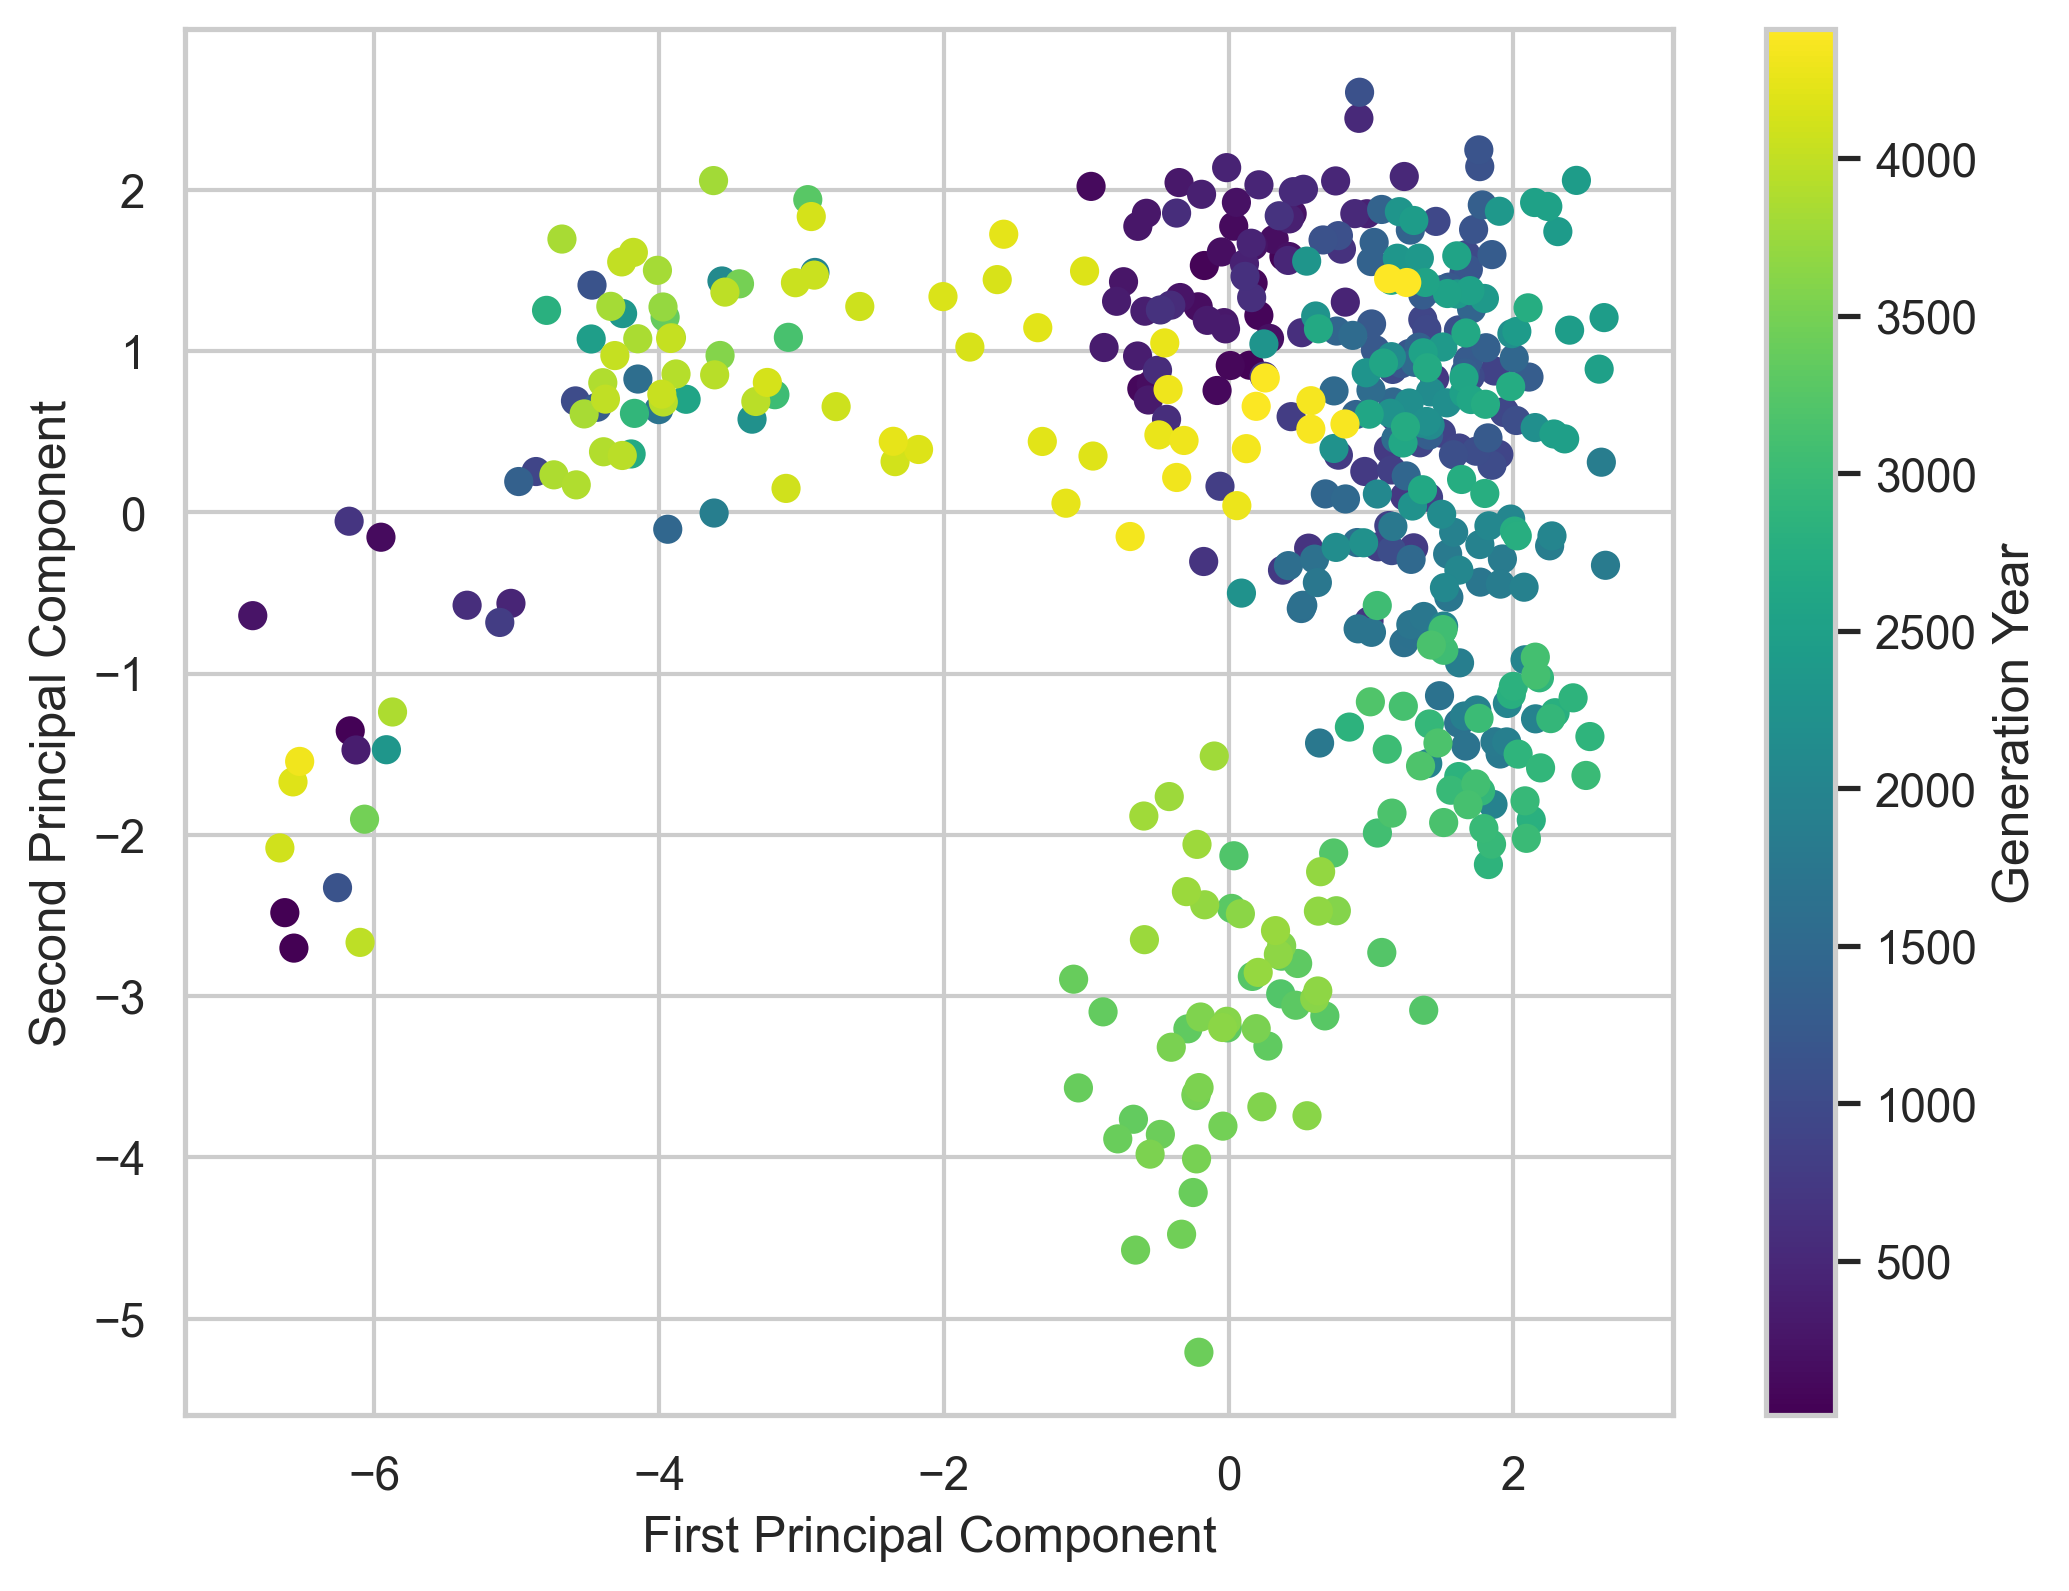
\includegraphics[width=\linewidth]{resources/partition_5_2906_3/partition_1/pca_scatterplot.png}
                    \textbf{Partition 1}
                \end{minipage}
                \hfill
                \begin{minipage}{0.32\textwidth}
                    \centering
                    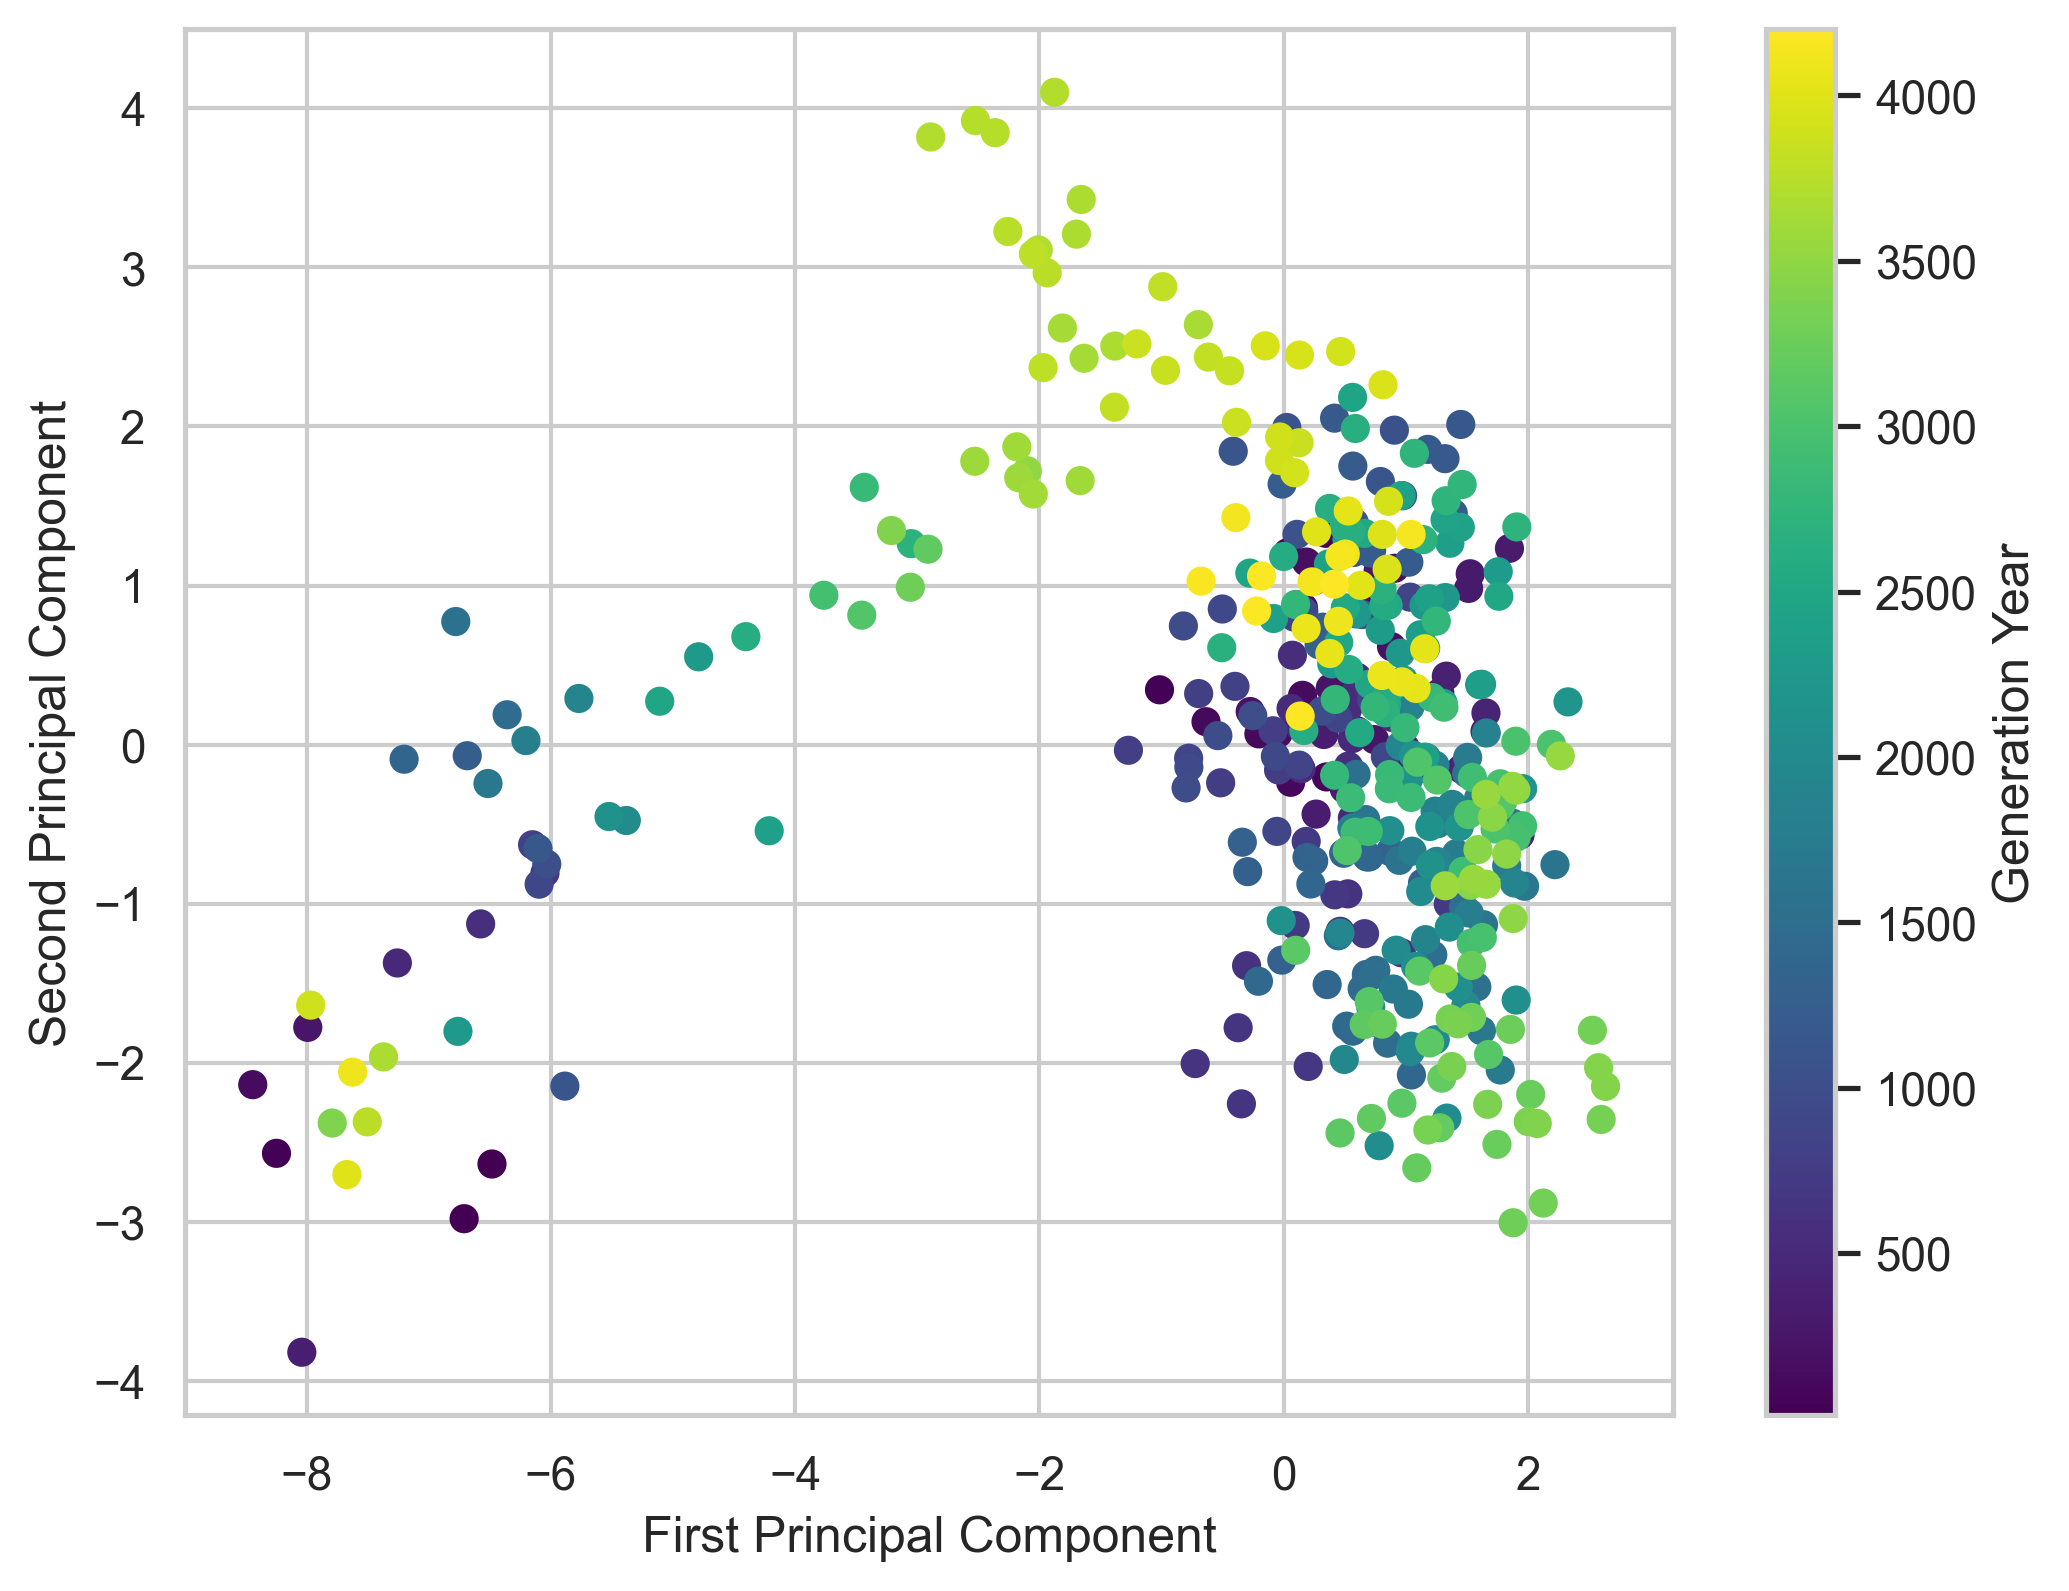
\includegraphics[width=\linewidth]{resources/partition_5_2906_3/partition_2/pca_scatterplot.png}
                    \textbf{Partition 2}
                \end{minipage}
                \caption{PCA scatterplots where the morphological parameters are reduced to 2 principal components.}
                \label{fig:pca_partition}
            \end{subfigure}

            \caption{Experiment 2 - Results of the second experiment where we evolve a set of generalist MC-pairs to handle a wide range of diverse environments.}
            \label{fig:experiment2}
        \end{figure*}

        Figure~\ref{fig:fit_heat_partitioned} shows the obtained fitness scores for each environment, represented in a heatmap for experiment 2. Similar to experiment 1, the hill environment shows high performance in the environments at the lower left, with relatively lower performance near the upper right. The fitness scores and their standard deviations for the training and testing sets are also similar. The training set has a mean fitness score of 3037.96 with a standard deviation of 1127.11, while the testing set has a mean fitness score of 3003.58 with a standard deviation of 1193.02. 

        For the rough terrain environment, the heatmap also shows high performance in the environments at the lower left and relatively lower performance near the upper right, and also in the lower right part, similar to experiment 1. The fitness scores on the training and testing sets are slightly different. The training set has a mean fitness score of 2812.58 with a standard deviation of 1016.59, and the testing set has a mean fitness score of 2679.42 with a standard deviation of 1215.64. 

        Overall, the set of MC-pairs do score a higher fitness on the rough terrain environment compared to experiment 1. This is evident when examining the partitions shown in figure~\ref{fig:heat_partition_number}. This figure presents the partitions to which each environment is assigned to. The blank white areas represent the testing environments that are not assigned to any partition. In this experiment, the environments in partition 1 and 2, that are being managed by another MC-pair, are of higher fitness scores, than in experiment one.

        The morphologies for each partition are visible in Figure~\ref{fig:part_ant_images}. The morphology in partition 0 is similar to the morphologies from experiment 1 in Figure~\ref{fig:gen_ant_images} with generalist scores 2412, 2784, and 3126. It also employs the same strategy to traverse the environment. This makes sense considering that experiment 1 is similar to the second experiment before partitioning. The morphology for partition 1 has two long front legs and two short back legs, where the back legs were used to propel itself, over the terrain. Lastly, the morphology in for partition 2 is comparatively smaller, featuring two back legs with thicker lower portions. It uses its front legs to latch onto a elevated terrain and subsequently try to climb it by then hooking its back legs to climb.

        The same PCA scatterplots where created for this experiment visible in Figure~\ref{fig:pca_partition}. These plots share many similarities with experiment 1 and do not reveal anything more compared to the plots from experiment 1.

    \subsection{Experiment 3: Specialist for each environment}
        \begin{figure*}[!ht]
            \centering
            \begin{subfigure}{\textwidth}
                \centering
                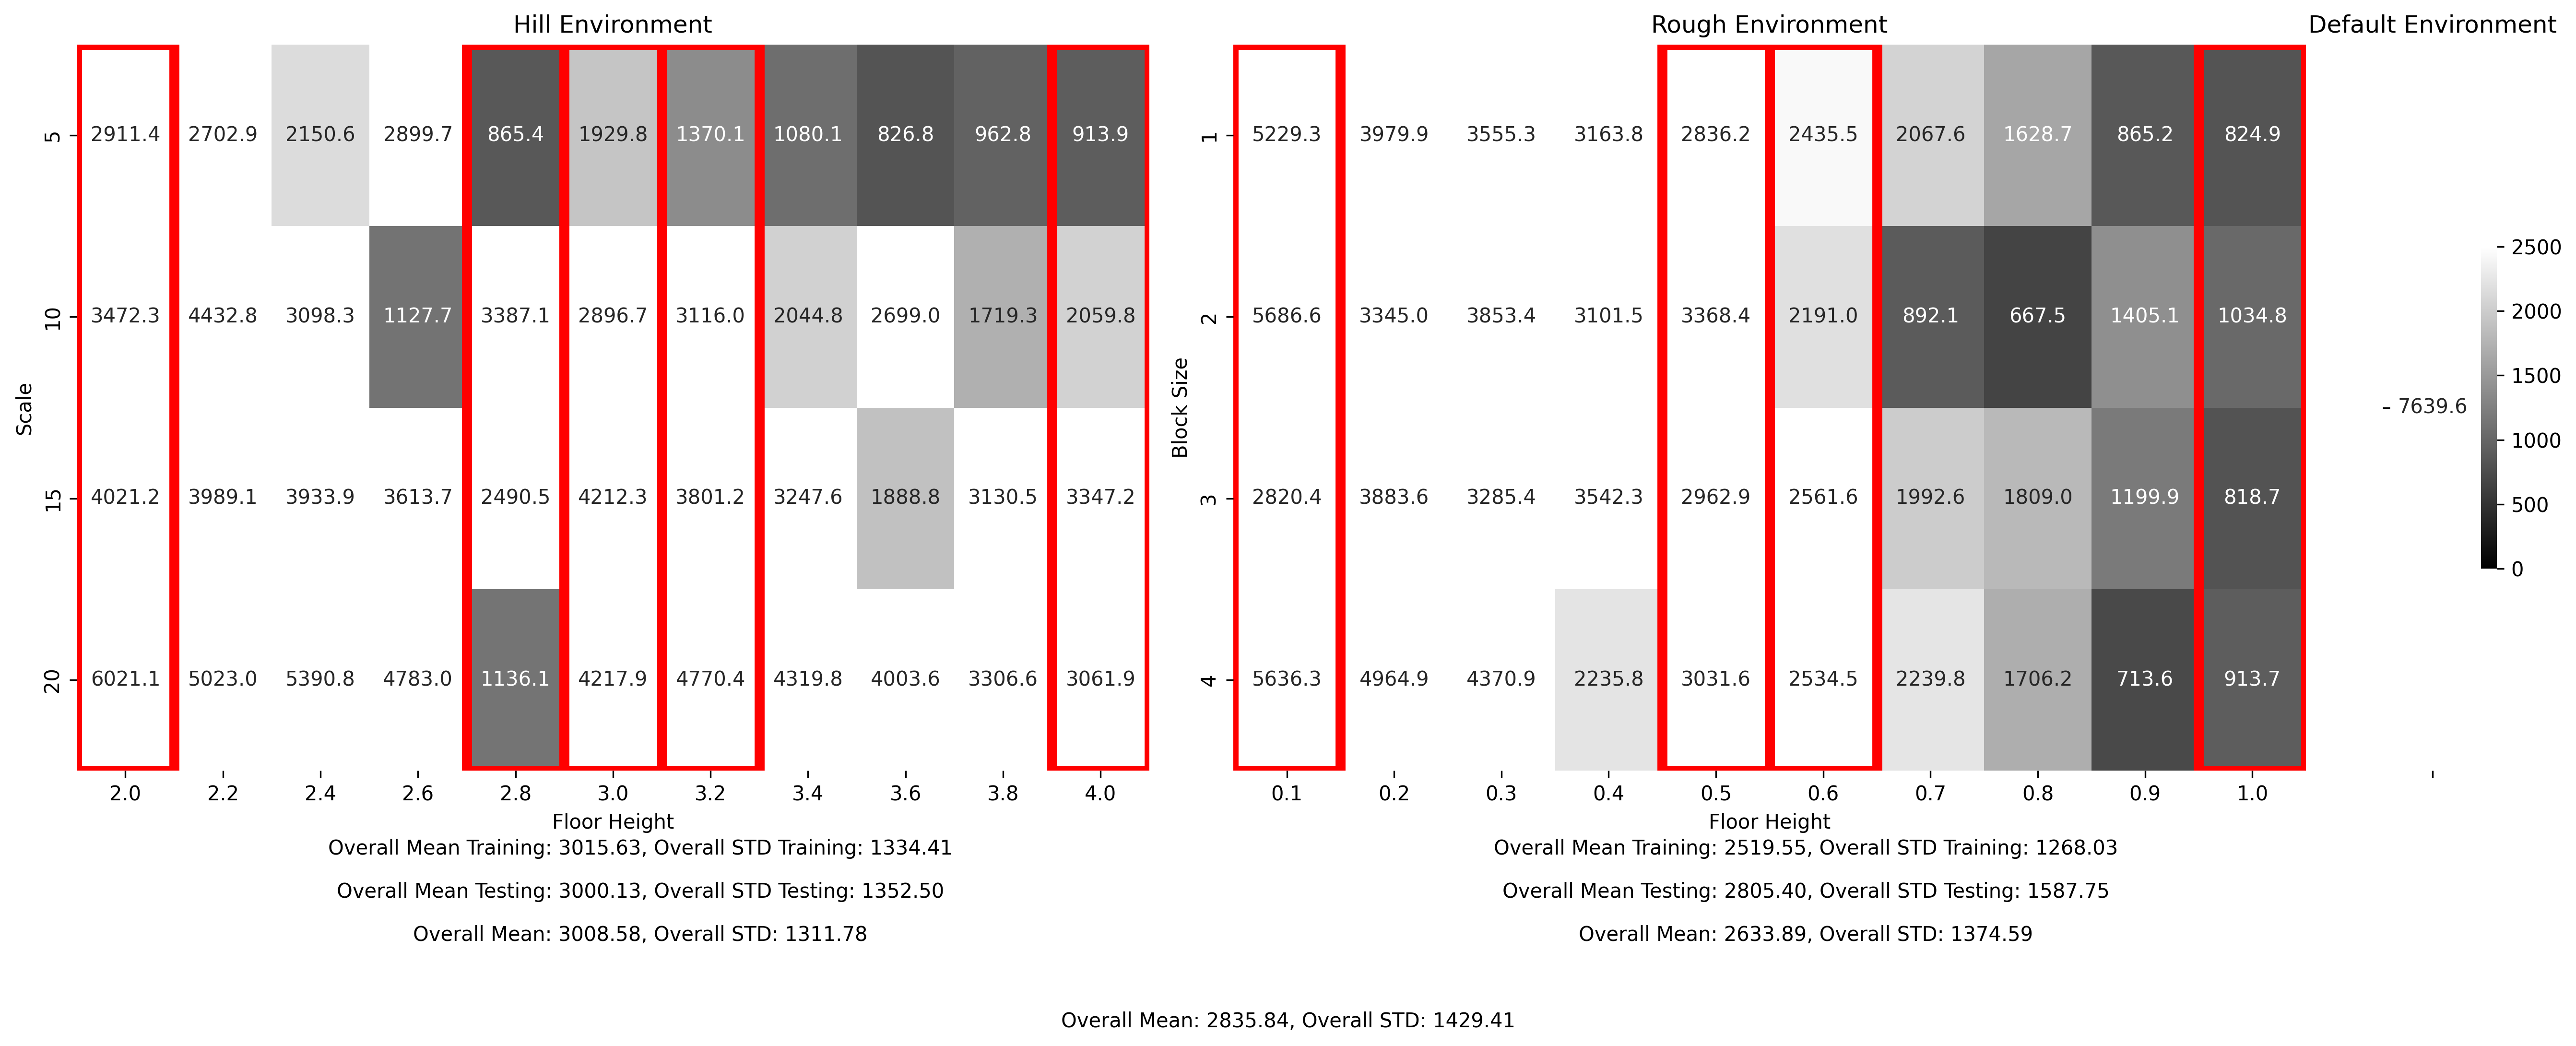
\includegraphics[width=\linewidth]{./resources/specialist_1_2835/fitness_heatmap.png}
                \caption{Fitness heatmap of a specialist MC-pair for each environment.}
                \label{fig:fit_heat_spec}
            \end{subfigure}

            \begin{subfigure}{\textwidth}
                \centering
                \begin{minipage}{0.19\textwidth}
                    \centering
                    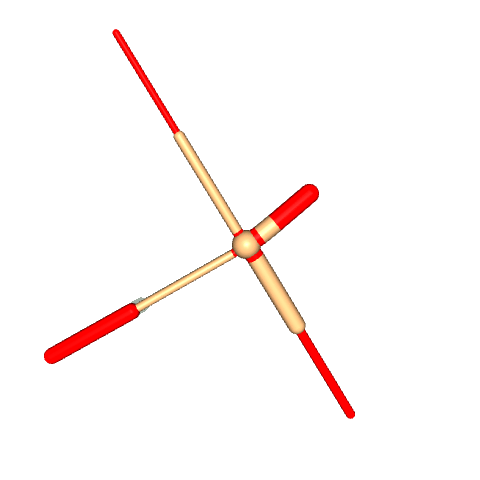
\includegraphics[width=\linewidth]{resources/specialist_1_2835/rough_4_0.4.png}
                    \textbf{Rough terrain Block size: 4 Floor height: 0.4}
                \end{minipage}
                \hfill
                \begin{minipage}{0.19\textwidth}
                    \centering
                    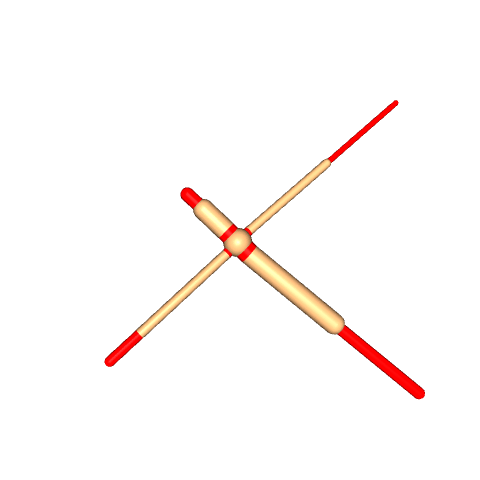
\includegraphics[width=\linewidth]{resources/specialist_1_2835/default.png}
                    \textbf{Default terrain}
                \end{minipage}
                \hfill
                \begin{minipage}{0.19\textwidth}
                    \centering
                    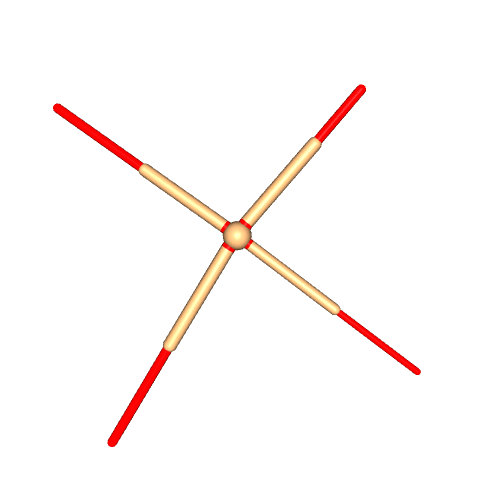
\includegraphics[width=\linewidth]{resources/specialist_1_2835/hills_20_2.0.png}
                    \textbf{Hills terrain Scale: 20 \newline Floor heigth: 2.0}
                \end{minipage}
                \caption{Specialist morphologies each evolved for one environment. The specific environment the morphology was evolved in is shown below the image.}
                \label{fig:spec_ant_images}
            \end{subfigure}

            \caption{Experiment 3 - Results of the third experiment where we evolve a specialist MC-pair for each individual environment.}
            \label{fig:experiment3}
        \end{figure*}

        Figure~\ref{fig:fit_heat_spec} shows the fitness scores obtained for each environment in experiment 3, represented as a heatmap. Unlike the results seen in experiment 1 and 2, this heatmap has a less distinct gradient. Fitness scores for some environments are lower than in the previous experiments, while others are higher. The overall mean fitness score across all environments is 2835.84 with a standard deviation of 1429.41. Although the is comparable to the previous experiments, the standard deviation is significantly greater, indicating more variability in the fitness scores. Notably, in the more complex environment, it was more challenging to evolve a performant specialist MC-pair, whilst the generalist scored higher. 
        
        Some interesting morphologies for some environments with unique strategies are showcased in Figure~\ref{fig:spec_ant_images}. The first morphology was evolved in the rough terrain environment with block size 4 and floor height 0.4. This terrain has larger size blocks elevated, requiring the ant's torso to be higher than the blocks in order to move forward. The long and thin leg was primarily used to lift the ant slightly into the air, while the other three legs were used to lunge itself forward. The second morphology was evolved in the default terrain environment. This terrain is completely flat, with no obstacles that could hinder the ant's forward motion. The two long and thin sidelegs are mainly responsible for the forward motion, while the longer front leg and very short back leg are mainly responsible for its balance. The front leg remains mostly still, only correcting the ant if it tips too far forward. The back leg does not touch the ground, but constantly makes a waggling movement. The third morphology was evolved in the hills terrain environment with scale 20 and floor height 2.0. The hills in this terrain are more stretched out and not as high, resembling a bit more to a flat environment. The ant looks almost symmetrical, with one leg bit longer then the rest. Each leg equally contributes to the forward movement, making it resemble an actual ants movement more. 




\section{Discussion}

\textbf{Interpretation of the result}

\textbf{Implications of the results}

In our experimental design, the starting position of the ant was set to one unit above the maximum floor height of the environment. This adjustment ensured that the ant would not spawn into the ground. However, this configuration introduced a minor delay in the ant's initial contact with the ground in environments with lower floor heights, thereby slightly disadvantaging them. However, this was not significantly noticable in the results, as the environments with lower floor heights are inherently easier than those with higher floor heights.

Another notable aspect of our experiment was the symmetry in the ant's morphology, which rendered modifications to  specific legs arbitrary. For instance, altering the length of legs 1 and 2 while shortening legs 3 and 4 results in the exact morphology to its reverse. This symmetry significantly reduced the number of novel morphologies the ant could evolve in drastically, despite a relatively large search space. To enhance the potential for more novel morphologies in future experiments, we could create and evolve the legs during the evolutionary process and include variations in the attachment points on the ant's torso for the leg. 

Given the diverse range of environments, each with unique challenges and complexities, employing TWEANNS might offer advantages over static ANN architectures. By using TWEANNS, it would be possible to evolve ANN structures specifically designed to generalize on all environments.

The methodology employed in this paper does not have an explicit objective function for generalizability; however, it emerges as a side effect of the applied methods. A future approach could involve making generalizability the primary objective. This approach would require increased computational resources, because of the need to assign a generalist score across the entire population, as also highlighted by Triebold et al. \cite{Corinna_Triebold}.

In our study, each type of environment was generated with just two dimensions. Adding additional dimensions will increase the variability of these environments, potentially further improving generalizability. Beyond solely structural modifications to the environment, incorporating variables such as changes in gravity or variations in the drag force of the ground could provide more insights into the evolution of MC-pairs, better mimicing real-world scenarios.
\section{Conclusion}

% References
\printbibliography

\end{document}